\documentclass[twoside]{book}

% Packages required by doxygen
\usepackage{calc}
\usepackage{doxygen}
\usepackage{graphicx}
\usepackage[utf8]{inputenc}
\usepackage{makeidx}
\usepackage{multicol}
\usepackage{multirow}
\PassOptionsToPackage{warn}{textcomp}
\usepackage{textcomp}
\usepackage[nointegrals]{wasysym}
\usepackage[table]{xcolor}

% NLS support packages
\usepackage{polski}
\usepackage[T1]{fontenc}

% Font selection
\usepackage[T1]{fontenc}
\usepackage{mathptmx}
\usepackage[scaled=.90]{helvet}
\usepackage{courier}
\usepackage{amssymb}
\usepackage{sectsty}
\renewcommand{\familydefault}{\sfdefault}
\allsectionsfont{%
  \fontseries{bc}\selectfont%
  \color{darkgray}%
}
\renewcommand{\DoxyLabelFont}{%
  \fontseries{bc}\selectfont%
  \color{darkgray}%
}
\newcommand{\+}{\discretionary{\mbox{\scriptsize$\hookleftarrow$}}{}{}}

% Page & text layout
\usepackage{geometry}
\geometry{%
  a4paper,%
  top=2.5cm,%
  bottom=2.5cm,%
  left=2.5cm,%
  right=2.5cm%
}
\tolerance=750
\hfuzz=15pt
\hbadness=750
\setlength{\emergencystretch}{15pt}
\setlength{\parindent}{0cm}
\setlength{\parskip}{0.2cm}
\makeatletter
\renewcommand{\paragraph}{%
  \@startsection{paragraph}{4}{0ex}{-1.0ex}{1.0ex}{%
    \normalfont\normalsize\bfseries\SS@parafont%
  }%
}
\renewcommand{\subparagraph}{%
  \@startsection{subparagraph}{5}{0ex}{-1.0ex}{1.0ex}{%
    \normalfont\normalsize\bfseries\SS@subparafont%
  }%
}
\makeatother

% Headers & footers
\usepackage{fancyhdr}
\pagestyle{fancyplain}
\fancyhead[LE]{\fancyplain{}{\bfseries\thepage}}
\fancyhead[CE]{\fancyplain{}{}}
\fancyhead[RE]{\fancyplain{}{\bfseries\leftmark}}
\fancyhead[LO]{\fancyplain{}{\bfseries\rightmark}}
\fancyhead[CO]{\fancyplain{}{}}
\fancyhead[RO]{\fancyplain{}{\bfseries\thepage}}
\fancyfoot[LE]{\fancyplain{}{}}
\fancyfoot[CE]{\fancyplain{}{}}
\fancyfoot[RE]{\fancyplain{}{\bfseries\scriptsize Wygenerowano N, 6 kwi 2014 23\+:43\+:26 dla Algorytmy Sortowania programem Doxygen }}
\fancyfoot[LO]{\fancyplain{}{\bfseries\scriptsize Wygenerowano N, 6 kwi 2014 23\+:43\+:26 dla Algorytmy Sortowania programem Doxygen }}
\fancyfoot[CO]{\fancyplain{}{}}
\fancyfoot[RO]{\fancyplain{}{}}
\renewcommand{\footrulewidth}{0.4pt}
\renewcommand{\chaptermark}[1]{%
  \markboth{#1}{}%
}
\renewcommand{\sectionmark}[1]{%
  \markright{\thesection\ #1}%
}

% Indices & bibliography
\usepackage{natbib}
\usepackage[titles]{tocloft}
\setcounter{tocdepth}{3}
\setcounter{secnumdepth}{5}
\makeindex

% Hyperlinks (required, but should be loaded last)
\usepackage{ifpdf}
\ifpdf
  \usepackage[pdftex,pagebackref=true]{hyperref}
\else
  \usepackage[ps2pdf,pagebackref=true]{hyperref}
\fi
\hypersetup{%
  colorlinks=true,%
  linkcolor=blue,%
  citecolor=blue,%
  unicode%
}

% Custom commands
\newcommand{\clearemptydoublepage}{%
  \newpage{\pagestyle{empty}\cleardoublepage}%
}


%===== C O N T E N T S =====

\begin{document}

% Titlepage & ToC
\hypersetup{pageanchor=false,
             bookmarks=true,
             bookmarksnumbered=true,
             pdfencoding=unicode
            }
\pagenumbering{roman}
\begin{titlepage}
\vspace*{7cm}
\begin{center}%
{\Large Algorytmy Sortowania \\[1ex]\large 2.\+0.\+5 }\\
\vspace*{1cm}
{\large Wygenerowano przez Doxygen 1.8.6}\\
\vspace*{0.5cm}
{\small N, 6 kwi 2014 23:43:26}\\
\end{center}
\end{titlepage}
\clearemptydoublepage
\tableofcontents
\clearemptydoublepage
\pagenumbering{arabic}
\hypersetup{pageanchor=true}

%--- Begin generated contents ---
\chapter{Indeks plików}
\section{Lista plików}
Tutaj znajduje się lista wszystkich plików z ich krótkimi opisami\+:\begin{DoxyCompactList}
\item\contentsline{section}{/home/administrator/\+P\+R\+O\+G\+R\+A\+M\+Y\+\_\+\+M\+A\+R\+Z\+E\+C\+\_\+2014/\+Sortowanie/\hyperlink{funkcje_8cpp}{funkcje.\+cpp} }{\pageref{funkcje_8cpp}}{}
\item\contentsline{section}{/home/administrator/\+P\+R\+O\+G\+R\+A\+M\+Y\+\_\+\+M\+A\+R\+Z\+E\+C\+\_\+2014/\+Sortowanie/\hyperlink{funkcje_8h}{funkcje.\+h} }{\pageref{funkcje_8h}}{}
\item\contentsline{section}{/home/administrator/\+P\+R\+O\+G\+R\+A\+M\+Y\+\_\+\+M\+A\+R\+Z\+E\+C\+\_\+2014/\+Sortowanie/\hyperlink{interfejs_8cpp}{interfejs.\+cpp} }{\pageref{interfejs_8cpp}}{}
\item\contentsline{section}{/home/administrator/\+P\+R\+O\+G\+R\+A\+M\+Y\+\_\+\+M\+A\+R\+Z\+E\+C\+\_\+2014/\+Sortowanie/\hyperlink{interfejs_8h}{interfejs.\+h} }{\pageref{interfejs_8h}}{}
\item\contentsline{section}{/home/administrator/\+P\+R\+O\+G\+R\+A\+M\+Y\+\_\+\+M\+A\+R\+Z\+E\+C\+\_\+2014/\+Sortowanie/\hyperlink{main_8cpp}{main.\+cpp} }{\pageref{main_8cpp}}{}
\end{DoxyCompactList}

\chapter{Dokumentacja plików}
\hypertarget{funkcje_8cpp}{\section{Dokumentacja pliku /home/administrator/\+P\+R\+O\+G\+R\+A\+M\+Y\+\_\+\+M\+A\+R\+Z\+E\+C\+\_\+2014/\+Sortowanie/funkcje.cpp}
\label{funkcje_8cpp}\index{/home/administrator/\+P\+R\+O\+G\+R\+A\+M\+Y\+\_\+\+M\+A\+R\+Z\+E\+C\+\_\+2014/\+Sortowanie/funkcje.\+cpp@{/home/administrator/\+P\+R\+O\+G\+R\+A\+M\+Y\+\_\+\+M\+A\+R\+Z\+E\+C\+\_\+2014/\+Sortowanie/funkcje.\+cpp}}
}
{\ttfamily \#include $<$iostream$>$}\\*
{\ttfamily \#include $<$time.\+h$>$}\\*
{\ttfamily \#include $<$cstdlib$>$}\\*
{\ttfamily \#include $<$iomanip$>$}\\*
{\ttfamily \#include $<$fstream$>$}\\*
{\ttfamily \#include $<$string$>$}\\*
{\ttfamily \#include $<$sstream$>$}\\*
Wykres zależności załączania dla funkcje.\+cpp\+:
\nopagebreak
\begin{figure}[H]
\begin{center}
\leavevmode
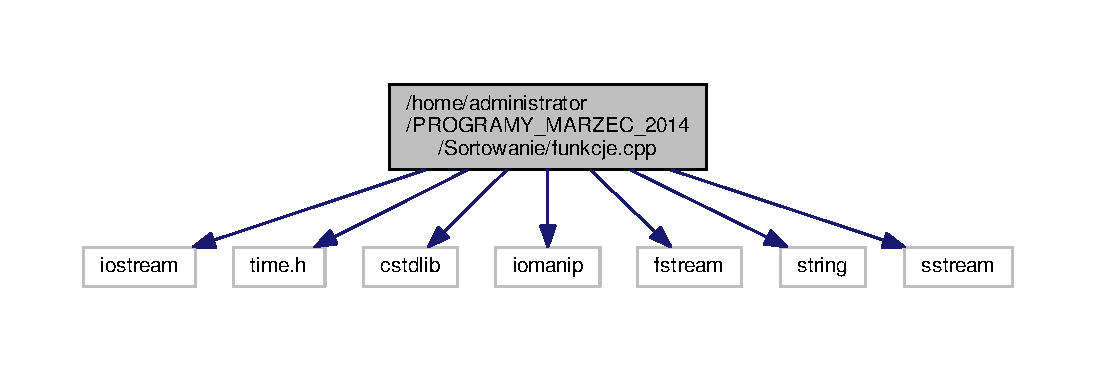
\includegraphics[width=350pt]{funkcje_8cpp__incl}
\end{center}
\end{figure}
\subsection*{Definicje}
\begin{DoxyCompactItemize}
\item 
\#define \hyperlink{funkcje_8cpp_aa806a6d84ea11a8548113d500356ae7f}{P\+R\+O\+G\+\_\+\+W\+I\+E\+L\+K\+O\+S\+C\+I\+\_\+\+T\+A\+B\+L\+I\+C\+Y}~64
\end{DoxyCompactItemize}
\subsection*{Funkcje}
\begin{DoxyCompactItemize}
\item 
int $\ast$ \hyperlink{funkcje_8cpp_ace17a33dbff93bc22f46764f0ed5ce88}{Stworz\+\_\+tablice} (int ilosc\+\_\+elementow)
\begin{DoxyCompactList}\small\item\em Funkcja tworzy pusta tablice (wypelniona N\+U\+L\+L'ami) z dynamiczna alokacja pamieci (wedle wyboru uzytkownika) \end{DoxyCompactList}\item 
int $\ast$ \hyperlink{funkcje_8cpp_a9f0b920042cd282ead67dc076d164916}{Stworz\+\_\+tablice} (int $\ast$T\+A\+B\+\_\+\+P\+O\+M, int ilosc\+\_\+elementow, int ile\+\_\+sortowac, int Z\+A\+K\+R\+E\+S\+\_\+\+L\+O\+S\+O\+W\+A\+N\+I\+A, int i)
\begin{DoxyCompactList}\small\item\em Funkcja tworzy tablice wypelniona {\itshape ilosc\+\_\+elementow} elementami z zakresu {\itshape Z\+A\+K\+R\+E\+S\+\_\+\+L\+O\+S\+O\+W\+A\+N\+I\+A}, a nastepnie sortuje czesc tablicy wedle ilosci {\itshape ile\+\_\+sortowac} \end{DoxyCompactList}\item 
void \hyperlink{funkcje_8cpp_a2527a77ab13de24d77e0a66680cd5abc}{P\+R\+Z\+Y\+P\+I\+S\+A\+N\+I\+E} (int $\ast$$\ast$T\+A\+B\+E\+L\+A\+\_\+\+S\+O\+R\+T\+O\+W\+A\+N, int $\ast$$\ast$T\+A\+B\+E\+L\+A, int ilosc\+\_\+elementow, int rozmiar\+\_\+tablicy)
\begin{DoxyCompactList}\small\item\em Funkcja przypisujaca wartosci tabeli pierwotnej (utworzonej przed rozpoczeciem sortowan) do tablicy, na ktorej wykonywane sa sortowania -\/ bez tej funkcji sortowanie odbywaloby sie tylko pierwszym algorytmem, a kolejne sortowalyby juz poukladana tabele. \end{DoxyCompactList}\item 
void \hyperlink{funkcje_8cpp_a3b14dea6d29a95e7c1cb103e00df39db}{Z\+A\+P\+I\+S\+\_\+\+C\+Z\+A\+S\+O\+W\+\_\+\+D\+O\+\_\+\+P\+L\+I\+K\+U} (double T\+A\+B\+E\+L\+A\+\_\+\+C\+Z\+A\+S\+O\+W\mbox{[}4\mbox{]}\mbox{[}100\mbox{]}, double T\+A\+B\+E\+L\+A\+\_\+\+C\+Z\+A\+S\+O\+W\+\_\+\+S\+U\+M\+Y\mbox{[}4\mbox{]}, int ilosc\+\_\+elementow, double ile\+\_\+posortowac, int zakres, int rozmiar\+\_\+petli)
\item 
void \hyperlink{funkcje_8cpp_a386f1a3ab0a1e37ec4c0d9df3ed0ebcc}{Sortowanie\+\_\+przez\+\_\+\+Scalanie} (int $\ast$T\+A\+B\+\_\+\+P\+O\+M, int $\ast$T\+A\+B\+L\+I\+C\+A, int lewy, int prawy)
\begin{DoxyCompactList}\small\item\em Algorytm sortowania przez scalanie. \end{DoxyCompactList}\item 
int \hyperlink{funkcje_8cpp_a1d774831882a4bac5c8012a1c0f44bfd}{Sortowanie\+\_\+\+Szybkie} (int $\ast$T\+A\+B\+L\+I\+C\+A, int lewy, int prawy, int P\+I\+W\+O\+T, bool introspektywne)
\begin{DoxyCompactList}\small\item\em Algorytm sortowanie szybkiego. \end{DoxyCompactList}\item 
void \hyperlink{funkcje_8cpp_afde57cb4cb5b41a2bdd32f85f94b2ddf}{Sortowanie\+\_\+\+Introspektywne} (int $\ast$T\+A\+B\+L\+I\+C\+A, int poczatek, int koniec, int L\+I\+M\+I\+T, bool introspektywne)
\begin{DoxyCompactList}\small\item\em Algorytm Sortowania Introspektywnego. \end{DoxyCompactList}\item 
void \hyperlink{funkcje_8cpp_af6adfabbbad6df1fec08f1ef1f856069}{Sortowanie\+\_\+\+Introspektywne\+\_\+petla} (int $\ast$T\+A\+B\+L\+I\+C\+A, int poczatek, int koniec, int L\+I\+M\+I\+T, bool introspektywne)
\item 
void \hyperlink{funkcje_8cpp_aa094b63bf46616da7c24d73c9cc0ca1e}{Sortowanie\+\_\+przez\+\_\+kopcowanie} (int $\ast$tablica, int lewy, int prawy)
\begin{DoxyCompactList}\small\item\em Algorytm sortowania przez kopcowanie. \end{DoxyCompactList}\item 
void \hyperlink{funkcje_8cpp_a62fc2c2ff60af5234f7a3163a52d1ff6}{Kopiec} (int $\ast$tablica, int poczatek, int koniec, int lewy)
\item 
int \hyperlink{funkcje_8cpp_abcf531366a1c7e8d850326e2a7480741}{N\+A\+J\+L\+E\+P\+S\+Z\+Y\+\_\+\+P\+I\+W\+O\+T} (int $\ast$T\+A\+B\+L\+I\+C\+A, int lewy, int srodek, int prawy)
\item 
string \hyperlink{funkcje_8cpp_a0a975119120cc8c23938545924c8f880}{Double\+\_\+na\+\_\+\+String} (double numer)
\item 
void \hyperlink{funkcje_8cpp_a1d73d0d6aa1c405560c9674351dcfca1}{Z\+A\+P\+I\+S\+\_\+\+C\+Z\+A\+S\+O\+W\+\_\+\+D\+O\+\_\+\+P\+L\+I\+K\+U} (double T\+A\+B\+E\+L\+A\+\_\+\+C\+Z\+A\+S\+O\+W\mbox{[}4\mbox{]}\mbox{[}100\mbox{]}, double T\+A\+B\+E\+L\+A\+\_\+\+C\+Z\+A\+S\+O\+W\+\_\+\+S\+U\+M\+Y\mbox{[}4\mbox{]}, int ilosc\+\_\+elementow, int wybor\+\_\+1, double ile\+\_\+posortowac, int wybor\+\_\+2, int zakres, int rozmiar\+\_\+petli)
\begin{DoxyCompactList}\small\item\em Funkcja zapisujaca czasy sortowan do plikow -\/ osobnych dla kazdego sortowania. \end{DoxyCompactList}\end{DoxyCompactItemize}


\subsection{Dokumentacja definicji}
\hypertarget{funkcje_8cpp_aa806a6d84ea11a8548113d500356ae7f}{\index{funkcje.\+cpp@{funkcje.\+cpp}!P\+R\+O\+G\+\_\+\+W\+I\+E\+L\+K\+O\+S\+C\+I\+\_\+\+T\+A\+B\+L\+I\+C\+Y@{P\+R\+O\+G\+\_\+\+W\+I\+E\+L\+K\+O\+S\+C\+I\+\_\+\+T\+A\+B\+L\+I\+C\+Y}}
\index{P\+R\+O\+G\+\_\+\+W\+I\+E\+L\+K\+O\+S\+C\+I\+\_\+\+T\+A\+B\+L\+I\+C\+Y@{P\+R\+O\+G\+\_\+\+W\+I\+E\+L\+K\+O\+S\+C\+I\+\_\+\+T\+A\+B\+L\+I\+C\+Y}!funkcje.\+cpp@{funkcje.\+cpp}}
\subsubsection[{P\+R\+O\+G\+\_\+\+W\+I\+E\+L\+K\+O\+S\+C\+I\+\_\+\+T\+A\+B\+L\+I\+C\+Y}]{\setlength{\rightskip}{0pt plus 5cm}\#define P\+R\+O\+G\+\_\+\+W\+I\+E\+L\+K\+O\+S\+C\+I\+\_\+\+T\+A\+B\+L\+I\+C\+Y~64}}\label{funkcje_8cpp_aa806a6d84ea11a8548113d500356ae7f}


\subsection{Dokumentacja funkcji}
\hypertarget{funkcje_8cpp_a0a975119120cc8c23938545924c8f880}{\index{funkcje.\+cpp@{funkcje.\+cpp}!Double\+\_\+na\+\_\+\+String@{Double\+\_\+na\+\_\+\+String}}
\index{Double\+\_\+na\+\_\+\+String@{Double\+\_\+na\+\_\+\+String}!funkcje.\+cpp@{funkcje.\+cpp}}
\subsubsection[{Double\+\_\+na\+\_\+\+String}]{\setlength{\rightskip}{0pt plus 5cm}string Double\+\_\+na\+\_\+\+String (
\begin{DoxyParamCaption}
\item[{double}]{numer}
\end{DoxyParamCaption}
)}}\label{funkcje_8cpp_a0a975119120cc8c23938545924c8f880}
\hypertarget{funkcje_8cpp_a62fc2c2ff60af5234f7a3163a52d1ff6}{\index{funkcje.\+cpp@{funkcje.\+cpp}!Kopiec@{Kopiec}}
\index{Kopiec@{Kopiec}!funkcje.\+cpp@{funkcje.\+cpp}}
\subsubsection[{Kopiec}]{\setlength{\rightskip}{0pt plus 5cm}void Kopiec (
\begin{DoxyParamCaption}
\item[{int $\ast$}]{tablica, }
\item[{int}]{poczatek, }
\item[{int}]{koniec, }
\item[{int}]{lewy}
\end{DoxyParamCaption}
)}}\label{funkcje_8cpp_a62fc2c2ff60af5234f7a3163a52d1ff6}
\hypertarget{funkcje_8cpp_abcf531366a1c7e8d850326e2a7480741}{\index{funkcje.\+cpp@{funkcje.\+cpp}!N\+A\+J\+L\+E\+P\+S\+Z\+Y\+\_\+\+P\+I\+W\+O\+T@{N\+A\+J\+L\+E\+P\+S\+Z\+Y\+\_\+\+P\+I\+W\+O\+T}}
\index{N\+A\+J\+L\+E\+P\+S\+Z\+Y\+\_\+\+P\+I\+W\+O\+T@{N\+A\+J\+L\+E\+P\+S\+Z\+Y\+\_\+\+P\+I\+W\+O\+T}!funkcje.\+cpp@{funkcje.\+cpp}}
\subsubsection[{N\+A\+J\+L\+E\+P\+S\+Z\+Y\+\_\+\+P\+I\+W\+O\+T}]{\setlength{\rightskip}{0pt plus 5cm}int N\+A\+J\+L\+E\+P\+S\+Z\+Y\+\_\+\+P\+I\+W\+O\+T (
\begin{DoxyParamCaption}
\item[{int $\ast$}]{T\+A\+B\+L\+I\+C\+A, }
\item[{int}]{lewy, }
\item[{int}]{srodek, }
\item[{int}]{prawy}
\end{DoxyParamCaption}
)}}\label{funkcje_8cpp_abcf531366a1c7e8d850326e2a7480741}
\hypertarget{funkcje_8cpp_a2527a77ab13de24d77e0a66680cd5abc}{\index{funkcje.\+cpp@{funkcje.\+cpp}!P\+R\+Z\+Y\+P\+I\+S\+A\+N\+I\+E@{P\+R\+Z\+Y\+P\+I\+S\+A\+N\+I\+E}}
\index{P\+R\+Z\+Y\+P\+I\+S\+A\+N\+I\+E@{P\+R\+Z\+Y\+P\+I\+S\+A\+N\+I\+E}!funkcje.\+cpp@{funkcje.\+cpp}}
\subsubsection[{P\+R\+Z\+Y\+P\+I\+S\+A\+N\+I\+E}]{\setlength{\rightskip}{0pt plus 5cm}void P\+R\+Z\+Y\+P\+I\+S\+A\+N\+I\+E (
\begin{DoxyParamCaption}
\item[{int $\ast$$\ast$}]{T\+A\+B\+E\+L\+A\+\_\+\+S\+O\+R\+T\+O\+W\+A\+N, }
\item[{int $\ast$$\ast$}]{T\+A\+B\+E\+L\+A, }
\item[{int}]{ilosc\+\_\+elementow, }
\item[{int}]{rozmiar\+\_\+tablicy}
\end{DoxyParamCaption}
)}}\label{funkcje_8cpp_a2527a77ab13de24d77e0a66680cd5abc}


Funkcja przypisujaca wartosci tabeli pierwotnej (utworzonej przed rozpoczeciem sortowan) do tablicy, na ktorej wykonywane sa sortowania -\/ bez tej funkcji sortowanie odbywaloby sie tylko pierwszym algorytmem, a kolejne sortowalyby juz poukladana tabele. 



 \subsubsection*{N\+A\+D\+P\+I\+S\+Y\+W\+A\+N\+I\+E T\+A\+B\+L\+I\+C\+Y I Z\+A\+P\+I\+S\+Y\+W\+A\+N\+I\+E }\hypertarget{funkcje_8cpp_afde57cb4cb5b41a2bdd32f85f94b2ddf}{\index{funkcje.\+cpp@{funkcje.\+cpp}!Sortowanie\+\_\+\+Introspektywne@{Sortowanie\+\_\+\+Introspektywne}}
\index{Sortowanie\+\_\+\+Introspektywne@{Sortowanie\+\_\+\+Introspektywne}!funkcje.\+cpp@{funkcje.\+cpp}}
\subsubsection[{Sortowanie\+\_\+\+Introspektywne}]{\setlength{\rightskip}{0pt plus 5cm}void Sortowanie\+\_\+\+Introspektywne (
\begin{DoxyParamCaption}
\item[{int $\ast$}]{T\+A\+B\+L\+I\+C\+A, }
\item[{int}]{poczatek, }
\item[{int}]{koniec, }
\item[{int}]{L\+I\+M\+I\+T, }
\item[{bool}]{introspektywne}
\end{DoxyParamCaption}
)}}\label{funkcje_8cpp_afde57cb4cb5b41a2bdd32f85f94b2ddf}


Algorytm Sortowania Introspektywnego. 

Funkcja Najpierw \char`\"{}dzieli\char`\"{} tablice kilka czesci i sortuje po kolei kolejne sekcje -\/ uzywajac sortowania przez kopcowanie. Po wstepnym posortowaniu tablicy zostaje ona poddana sortowaniu szybkiemu (ze wskazanym Piwotem wyznaczonym przez funkcje N\+A\+J\+L\+E\+P\+S\+Z\+Y\+\_\+\+P\+I\+W\+O\+T). Nastepnie wywolywana jest rekurencyjnie petla sortowania introspektywnego, a numer elementu na ktorym zostalo zakonczone dane sortowanie jest okreslana przez numer elementu zwracany przez sortowanie szybkie. Po podziale tablicy na mniej niz (64 elementy) sortowanie dopelnia sortowanie przez wstawianie -\/ ktore dziala bardzo dobrze dla prawie posortowanych tabel


\begin{DoxyParams}{Parametry}
{\em T\+A\+B\+L\+I\+C\+A} & -\/ Tablica (jeden wiersz) zawieracajaca sortowany zestaw liczb \\
\hline
{\em poczatek} & -\/ poczatek podzialu tablicy -\/ wskaznik na element tablicy przekazywany do petli Introsorta \\
\hline
{\em koniec} & -\/ koniec podzialu tablicy \\
\hline
{\em L\+I\+M\+I\+T} & -\/ tablica jest wstepnie sortowana przez algorytm sortowania przez kopcowanie, a gdy zostanie posortowana do pewnego stopnia, zostaje przekazana do sortowania szybkiego \\
\hline
{\em introspektywne} & -\/ zmienna decydujaca jak ma dzialac sortowanie szybkie \\
\hline
\end{DoxyParams}
Sortowanie\+\_\+\+Introspektywne\+\_\+petla zawieta sortowania przez kopcowanie i sortowanie szybkie

Dokonczenie skladania / sortowania tablicy poprzez proste sortowanie przez wstawianie \hypertarget{funkcje_8cpp_af6adfabbbad6df1fec08f1ef1f856069}{\index{funkcje.\+cpp@{funkcje.\+cpp}!Sortowanie\+\_\+\+Introspektywne\+\_\+petla@{Sortowanie\+\_\+\+Introspektywne\+\_\+petla}}
\index{Sortowanie\+\_\+\+Introspektywne\+\_\+petla@{Sortowanie\+\_\+\+Introspektywne\+\_\+petla}!funkcje.\+cpp@{funkcje.\+cpp}}
\subsubsection[{Sortowanie\+\_\+\+Introspektywne\+\_\+petla}]{\setlength{\rightskip}{0pt plus 5cm}void Sortowanie\+\_\+\+Introspektywne\+\_\+petla (
\begin{DoxyParamCaption}
\item[{int $\ast$}]{T\+A\+B\+L\+I\+C\+A, }
\item[{int}]{poczatek, }
\item[{int}]{koniec, }
\item[{int}]{L\+I\+M\+I\+T, }
\item[{bool}]{introspektywne}
\end{DoxyParamCaption}
)}}\label{funkcje_8cpp_af6adfabbbad6df1fec08f1ef1f856069}


 \subsubsection*{F\+U\+N\+K\+C\+J\+E I\+N\+T\+R\+O\+S\+O\+R\+T\+A + S\+O\+R\+T\+O\+W\+A\+N\+I\+E P\+R\+Z\+E\+Z K\+O\+P\+C\+O\+W\+A\+N\+I\+E }\hypertarget{funkcje_8cpp_aa094b63bf46616da7c24d73c9cc0ca1e}{\index{funkcje.\+cpp@{funkcje.\+cpp}!Sortowanie\+\_\+przez\+\_\+kopcowanie@{Sortowanie\+\_\+przez\+\_\+kopcowanie}}
\index{Sortowanie\+\_\+przez\+\_\+kopcowanie@{Sortowanie\+\_\+przez\+\_\+kopcowanie}!funkcje.\+cpp@{funkcje.\+cpp}}
\subsubsection[{Sortowanie\+\_\+przez\+\_\+kopcowanie}]{\setlength{\rightskip}{0pt plus 5cm}void Sortowanie\+\_\+przez\+\_\+kopcowanie (
\begin{DoxyParamCaption}
\item[{int $\ast$}]{tablica, }
\item[{int}]{lewy, }
\item[{int}]{prawy}
\end{DoxyParamCaption}
)}}\label{funkcje_8cpp_aa094b63bf46616da7c24d73c9cc0ca1e}


Algorytm sortowania przez kopcowanie. 


\begin{DoxyParams}{Parametry}
{\em tablica} & -\/ Tablica (jeden wiersz) zawieracajaca sortowany zestaw liczb \\
\hline
{\em lewy} & -\/ wskaznik (nr elementu) lewej granicy sortowanej czesci tablicy \\
\hline
{\em prawy} & -\/ wskaznik (nr elementu) prawej granicy sortowanej czesci tablicy \\
\hline
\end{DoxyParams}
\hypertarget{funkcje_8cpp_a386f1a3ab0a1e37ec4c0d9df3ed0ebcc}{\index{funkcje.\+cpp@{funkcje.\+cpp}!Sortowanie\+\_\+przez\+\_\+\+Scalanie@{Sortowanie\+\_\+przez\+\_\+\+Scalanie}}
\index{Sortowanie\+\_\+przez\+\_\+\+Scalanie@{Sortowanie\+\_\+przez\+\_\+\+Scalanie}!funkcje.\+cpp@{funkcje.\+cpp}}
\subsubsection[{Sortowanie\+\_\+przez\+\_\+\+Scalanie}]{\setlength{\rightskip}{0pt plus 5cm}void Sortowanie\+\_\+przez\+\_\+\+Scalanie (
\begin{DoxyParamCaption}
\item[{int $\ast$}]{T\+A\+B\+\_\+\+P\+O\+M, }
\item[{int $\ast$}]{T\+A\+B\+L\+I\+C\+A, }
\item[{int}]{lewy, }
\item[{int}]{prawy}
\end{DoxyParamCaption}
)}}\label{funkcje_8cpp_a386f1a3ab0a1e37ec4c0d9df3ed0ebcc}


Algorytm sortowania przez scalanie. 



 \subsubsection*{S\+O\+R\+T\+O\+W\+A\+N\+I\+A\+: S\+C\+A\+L\+A\+N\+I\+E / Q\+U\+I\+C\+K\+S\+O\+R\+T / I\+N\+T\+R\+O\+S\+P\+E\+K\+T\+Y\+W\+N\+E }inicjalizacja zmiennych

wybor srodkowego elementu danego podzialu

Dziel rekurencyjnie

Inicjalizacja wskaznikow / tymczasowych wartosci elementow lewy i srodek I rozpoczecie procedury sortowania elementow w \char`\"{}podtablicach\char`\"{}

Przypisanie posortowanych elementow do tablicy glownej\hypertarget{funkcje_8cpp_a1d774831882a4bac5c8012a1c0f44bfd}{\index{funkcje.\+cpp@{funkcje.\+cpp}!Sortowanie\+\_\+\+Szybkie@{Sortowanie\+\_\+\+Szybkie}}
\index{Sortowanie\+\_\+\+Szybkie@{Sortowanie\+\_\+\+Szybkie}!funkcje.\+cpp@{funkcje.\+cpp}}
\subsubsection[{Sortowanie\+\_\+\+Szybkie}]{\setlength{\rightskip}{0pt plus 5cm}int Sortowanie\+\_\+\+Szybkie (
\begin{DoxyParamCaption}
\item[{int $\ast$}]{T\+A\+B\+L\+I\+C\+A, }
\item[{int}]{lewy, }
\item[{int}]{prawy, }
\item[{int}]{P\+I\+W\+O\+T, }
\item[{bool}]{introspektywne}
\end{DoxyParamCaption}
)}}\label{funkcje_8cpp_a1d774831882a4bac5c8012a1c0f44bfd}


Algorytm sortowanie szybkiego. 

Do funkcji przekazywana jest tablica (jeden wiersz), a nastepnie wykonywany jest na niej algorytm sortowania szybkiego. Funkcja ta jest rowniez wykozystywana podczas sortowania introspektywnego -\/ stad zmienna bool introspektywne. Funkcja dzieli tablice wg. Piwotu -\/ dla introspektywnego okreslany wg algorytmu wyboru Piwotu, dla szybkiego testy wykazaly, ze szybszy jest podzial tablicy na pol.

Nastepnie poprawnosc polozenia elementu w tablicy jest sprawdzany -\/ jezeli jest po \char`\"{}zlej stronie\char`\"{} liczby okreslajacej srodek tablicy (piwot) zostaja zamienione -\/ jezeli nie to przesuwany jest wskaznik lewego i prawego elementu do czasu znalezienia takiej \char`\"{}pary\char`\"{}. Nastepnie wstepnie posortowana tablica jest dzielona na mniejsze, az do rozbicia na najmniejsze mozliwe podtablice


\begin{DoxyParams}{Parametry}
{\em T\+A\+B\+L\+I\+C\+A} & -\/ Tablica (jeden wiersz) zawieracajaca sortowany zestaw liczb \\
\hline
{\em lewy} & -\/ Wartosc lewego elementu \\
\hline
{\em prawy} & -\/ Wartosc prawego elementu \\
\hline
{\em P\+I\+W\+O\+T} & -\/ Zmienna uzywana przez sortowanie introspektywne. Element podzialu tablicy jest wybierany na podstawie algorytmu \\
\hline
{\em introspektywne} & -\/ okresla jak uzywac sortowania szybkiego -\/ implementacja dla sortowania introspektywnego nieco rozni sie niz w przypadku sortowania szybkiego \\
\hline
\end{DoxyParams}
\begin{DoxyReturn}{Zwraca}
int -\/ Zwraca posortowany wiersz tablicy do petli glownej programu 
\end{DoxyReturn}
czy uzyc sortowania jako czesci introspektywnego -\/ okreslenie Piwotu

jezeli nie to wskaz srodek jako optymalny piwot

przypisanie wskaznika (w formie wartosci) dla przegladania tablicy

dopuki nie sprawdzi calej tablicy

dopuki element mniejszy od piwotu, zwiekszaj numer elementu az trafisz na wiekszy od niego

dopuki element wiekszy od piwotu, zmniejszaj numer elementu az trafisz na mniejszy od niego

zamien oba nie pasujace elementy ze soba miejscami

i przesun sie do kolejnych elementow

jezeli elementy beda rowne sobie (dojda do \char`\"{}piwotu\char`\"{}) to zwroc (dla introspektywnego) wskaznik na lewy element lub przerwij petle \hypertarget{funkcje_8cpp_ace17a33dbff93bc22f46764f0ed5ce88}{\index{funkcje.\+cpp@{funkcje.\+cpp}!Stworz\+\_\+tablice@{Stworz\+\_\+tablice}}
\index{Stworz\+\_\+tablice@{Stworz\+\_\+tablice}!funkcje.\+cpp@{funkcje.\+cpp}}
\subsubsection[{Stworz\+\_\+tablice}]{\setlength{\rightskip}{0pt plus 5cm}int $\ast$ Stworz\+\_\+tablice (
\begin{DoxyParamCaption}
\item[{int}]{ilosc\+\_\+elementow}
\end{DoxyParamCaption}
)}}\label{funkcje_8cpp_ace17a33dbff93bc22f46764f0ed5ce88}


Funkcja tworzy pusta tablice (wypelniona N\+U\+L\+L'ami) z dynamiczna alokacja pamieci (wedle wyboru uzytkownika) 



 \subsubsection*{T\+W\+O\+R\+Z\+E\+N\+I\+E T\+A\+B\+L\+I\+C }\hypertarget{funkcje_8cpp_a9f0b920042cd282ead67dc076d164916}{\index{funkcje.\+cpp@{funkcje.\+cpp}!Stworz\+\_\+tablice@{Stworz\+\_\+tablice}}
\index{Stworz\+\_\+tablice@{Stworz\+\_\+tablice}!funkcje.\+cpp@{funkcje.\+cpp}}
\subsubsection[{Stworz\+\_\+tablice}]{\setlength{\rightskip}{0pt plus 5cm}int $\ast$ Stworz\+\_\+tablice (
\begin{DoxyParamCaption}
\item[{int $\ast$}]{T\+A\+B\+\_\+\+P\+O\+M, }
\item[{int}]{ilosc\+\_\+elementow, }
\item[{int}]{ile\+\_\+sortowac, }
\item[{int}]{Z\+A\+K\+R\+E\+S\+\_\+\+L\+O\+S\+O\+W\+A\+N\+I\+A, }
\item[{int}]{i}
\end{DoxyParamCaption}
)}}\label{funkcje_8cpp_a9f0b920042cd282ead67dc076d164916}


Funkcja tworzy tablice wypelniona {\itshape ilosc\+\_\+elementow} elementami z zakresu {\itshape Z\+A\+K\+R\+E\+S\+\_\+\+L\+O\+S\+O\+W\+A\+N\+I\+A}, a nastepnie sortuje czesc tablicy wedle ilosci {\itshape ile\+\_\+sortowac} 


\begin{DoxyParams}{Parametry}
{\em T\+A\+B\+\_\+\+P\+O\+M} & -\/ Tablica pomocnicza (pierwotnie pusta) przekazywana do funkcji tylko w celu sortowania wstepnego -\/ wymagana do sortowania przez scalanie -\/ algorytmu wykozystanego do posortowania wstepnego tablicy \\
\hline
{\em ilosc\+\_\+elementow} & -\/ ilosc elementow okreslona przez uzytkownika, okresla wielkosc tworzonej tablicy \\
\hline
{\em ile\+\_\+sortowac} & -\/ sortowanie wstepne tablicy elementow \\
\hline
{\em Z\+A\+K\+R\+E\+S\+\_\+\+L\+O\+S\+O\+W\+A\+N\+I\+A} & -\/ zakres (0 -\/ x) -\/ przedzial, z ktorego losowane beda liczby do danej tablicy \\
\hline
{\em i} & -\/ jako ze do program tworzy od razu 100 takich tabel (dla lepszej analizy dzialania algorytmow), przekazywany jest numer aktualnie tworzonej tablicy -\/ dodanie go do R\+A\+N\+D'a podczas losowania liczb zapobiega utworzeniu dwoch takich samych tabel obok siebie \\
\hline
\end{DoxyParams}
\begin{DoxyReturn}{Zwraca}
int -\/ zwraca tablice (w formie tablicy jednowymiarowej o wielkosci $\ast$\mbox{[}ilosc\+\_\+elementow\mbox{]}$\ast$ i przypisuje ja jako dany wiersz tablicy dwuwymiarowej o rozmiarze $\ast$\mbox{[}100\mbox{]}\mbox{[}ilosc\+\_\+elementow\mbox{]}$\ast$ w petli glownej programu 
\end{DoxyReturn}
\hypertarget{funkcje_8cpp_a3b14dea6d29a95e7c1cb103e00df39db}{\index{funkcje.\+cpp@{funkcje.\+cpp}!Z\+A\+P\+I\+S\+\_\+\+C\+Z\+A\+S\+O\+W\+\_\+\+D\+O\+\_\+\+P\+L\+I\+K\+U@{Z\+A\+P\+I\+S\+\_\+\+C\+Z\+A\+S\+O\+W\+\_\+\+D\+O\+\_\+\+P\+L\+I\+K\+U}}
\index{Z\+A\+P\+I\+S\+\_\+\+C\+Z\+A\+S\+O\+W\+\_\+\+D\+O\+\_\+\+P\+L\+I\+K\+U@{Z\+A\+P\+I\+S\+\_\+\+C\+Z\+A\+S\+O\+W\+\_\+\+D\+O\+\_\+\+P\+L\+I\+K\+U}!funkcje.\+cpp@{funkcje.\+cpp}}
\subsubsection[{Z\+A\+P\+I\+S\+\_\+\+C\+Z\+A\+S\+O\+W\+\_\+\+D\+O\+\_\+\+P\+L\+I\+K\+U}]{\setlength{\rightskip}{0pt plus 5cm}void Z\+A\+P\+I\+S\+\_\+\+C\+Z\+A\+S\+O\+W\+\_\+\+D\+O\+\_\+\+P\+L\+I\+K\+U (
\begin{DoxyParamCaption}
\item[{double}]{T\+A\+B\+E\+L\+A\+\_\+\+C\+Z\+A\+S\+O\+W\mbox{[}4\mbox{]}\mbox{[}100\mbox{]}, }
\item[{double}]{T\+A\+B\+E\+L\+A\+\_\+\+C\+Z\+A\+S\+O\+W\+\_\+\+S\+U\+M\+Y\mbox{[}4\mbox{]}, }
\item[{int}]{ilosc\+\_\+elementow, }
\item[{double}]{ile\+\_\+posortowac, }
\item[{int}]{zakres, }
\item[{int}]{rozmiar\+\_\+petli}
\end{DoxyParamCaption}
)}}\label{funkcje_8cpp_a3b14dea6d29a95e7c1cb103e00df39db}
\hypertarget{funkcje_8cpp_a1d73d0d6aa1c405560c9674351dcfca1}{\index{funkcje.\+cpp@{funkcje.\+cpp}!Z\+A\+P\+I\+S\+\_\+\+C\+Z\+A\+S\+O\+W\+\_\+\+D\+O\+\_\+\+P\+L\+I\+K\+U@{Z\+A\+P\+I\+S\+\_\+\+C\+Z\+A\+S\+O\+W\+\_\+\+D\+O\+\_\+\+P\+L\+I\+K\+U}}
\index{Z\+A\+P\+I\+S\+\_\+\+C\+Z\+A\+S\+O\+W\+\_\+\+D\+O\+\_\+\+P\+L\+I\+K\+U@{Z\+A\+P\+I\+S\+\_\+\+C\+Z\+A\+S\+O\+W\+\_\+\+D\+O\+\_\+\+P\+L\+I\+K\+U}!funkcje.\+cpp@{funkcje.\+cpp}}
\subsubsection[{Z\+A\+P\+I\+S\+\_\+\+C\+Z\+A\+S\+O\+W\+\_\+\+D\+O\+\_\+\+P\+L\+I\+K\+U}]{\setlength{\rightskip}{0pt plus 5cm}void Z\+A\+P\+I\+S\+\_\+\+C\+Z\+A\+S\+O\+W\+\_\+\+D\+O\+\_\+\+P\+L\+I\+K\+U (
\begin{DoxyParamCaption}
\item[{double}]{T\+A\+B\+E\+L\+A\+\_\+\+C\+Z\+A\+S\+O\+W\mbox{[}4\mbox{]}\mbox{[}100\mbox{]}, }
\item[{double}]{T\+A\+B\+E\+L\+A\+\_\+\+C\+Z\+A\+S\+O\+W\+\_\+\+S\+U\+M\+Y\mbox{[}4\mbox{]}, }
\item[{int}]{ilosc\+\_\+elementow, }
\item[{int}]{wybor\+\_\+1, }
\item[{double}]{ile\+\_\+posortowac, }
\item[{int}]{wybor\+\_\+2, }
\item[{int}]{zakres, }
\item[{int}]{rozmiar\+\_\+petli}
\end{DoxyParamCaption}
)}}\label{funkcje_8cpp_a1d73d0d6aa1c405560c9674351dcfca1}


Funkcja zapisujaca czasy sortowan do plikow -\/ osobnych dla kazdego sortowania. 


\begin{DoxyParams}{Parametry}
{\em T\+A\+B\+E\+L\+A\+\_\+\+C\+Z\+A\+S\+O\+W\mbox{[}$\,$\mbox{]}\mbox{[}$\,$\mbox{]}} & -\/ przechowuje czasy sortowania poszczegolnego wiersza
\begin{DoxyEnumerate}
\item Rozmiar Y -\/ czasy poszczegolnego sortowania
\item Rozmiar X -\/ czas sortowania kazdego wiersza tabeli 
\end{DoxyEnumerate}\\
\hline
{\em T\+A\+B\+E\+L\+A\+\_\+\+C\+Z\+A\+S\+O\+W\+\_\+\+S\+U\+M\+Y\mbox{[}$\,$\mbox{]}} & -\/ Czas wykonania kazdego algorytmu (suma czasow wykonania sortowan na 100 tablicach) \\
\hline
{\em ilosc\+\_\+elementow} & -\/ ilosc elementow kazdej tablicy \\
\hline
{\em wybor\+\_\+1} & -\/ przekazywana w celu okreslenia nazwy pliku wynikowego \\
\hline
{\em ile\+\_\+posortowac} & -\/ ilosc wstepnie posortowanych elementow \\
\hline
{\em wybor\+\_\+2} & -\/ okreslenie ilosci posortowanych elementow -\/ do nazwy pliku \\
\hline
{\em zakres} & -\/ zakres (0 -\/ x), z ktorego losowane sa liczby w tablicach \\
\hline
{\em rozmiar\+\_\+petli} & -\/ ilosc wierszy (instancji tablic) do sortowania \\
\hline
\end{DoxyParams}

\hypertarget{funkcje_8h}{\section{Dokumentacja pliku /home/administrator/\+P\+R\+O\+G\+R\+A\+M\+Y\+\_\+\+M\+A\+R\+Z\+E\+C\+\_\+2014/\+Sortowanie/funkcje.h}
\label{funkcje_8h}\index{/home/administrator/\+P\+R\+O\+G\+R\+A\+M\+Y\+\_\+\+M\+A\+R\+Z\+E\+C\+\_\+2014/\+Sortowanie/funkcje.\+h@{/home/administrator/\+P\+R\+O\+G\+R\+A\+M\+Y\+\_\+\+M\+A\+R\+Z\+E\+C\+\_\+2014/\+Sortowanie/funkcje.\+h}}
}
Ten wykres pokazuje, które pliki bezpośrednio lub pośrednio załączają ten plik\+:
\nopagebreak
\begin{figure}[H]
\begin{center}
\leavevmode
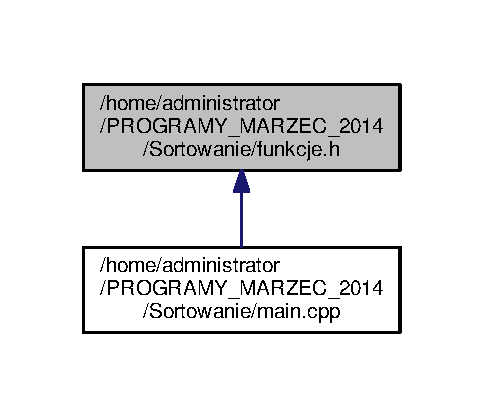
\includegraphics[width=232pt]{funkcje_8h__dep__incl}
\end{center}
\end{figure}
\subsection*{Funkcje}
\begin{DoxyCompactItemize}
\item 
int $\ast$ \hyperlink{funkcje_8h_a6c0696838db286457e2615cd27971459}{Stworz\+\_\+tablice} (int ilosc\+\_\+elementow)
\begin{DoxyCompactList}\small\item\em Funkcja tworzy pusta tablice (wypelniona N\+U\+L\+L'ami) z dynamiczna alokacja pamieci (wedle wyboru uzytkownika) \end{DoxyCompactList}\item 
int $\ast$ \hyperlink{funkcje_8h_a7e56db3d1f68f3c8f0b7f3171c18b2c5}{Stworz\+\_\+tablice} (int $\ast$T\+A\+B\+\_\+\+P\+O\+M, int ilosc\+\_\+elementow, int ile\+\_\+sortowac, int Z\+A\+K\+R\+E\+S\+\_\+\+L\+O\+S\+O\+W\+A\+N\+I\+A, int i)
\begin{DoxyCompactList}\small\item\em Funkcja tworzy tablice wypelniona {\itshape ilosc\+\_\+elementow} elementami z zakresu {\itshape Z\+A\+K\+R\+E\+S\+\_\+\+L\+O\+S\+O\+W\+A\+N\+I\+A}, a nastepnie sortuje czesc tablicy wedle ilosci {\itshape ile\+\_\+sortowac} \end{DoxyCompactList}\item 
void \hyperlink{funkcje_8h_a2527a77ab13de24d77e0a66680cd5abc}{P\+R\+Z\+Y\+P\+I\+S\+A\+N\+I\+E} (int $\ast$$\ast$T\+A\+B\+E\+L\+A\+\_\+\+S\+O\+R\+T\+O\+W\+A\+N, int $\ast$$\ast$T\+A\+B\+E\+L\+A, int ilosc\+\_\+elementow, int rozmiar\+\_\+tablicy)
\begin{DoxyCompactList}\small\item\em Funkcja przypisujaca wartosci tabeli pierwotnej (utworzonej przed rozpoczeciem sortowan) do tablicy, na ktorej wykonywane sa sortowania -\/ bez tej funkcji sortowanie odbywaloby sie tylko pierwszym algorytmem, a kolejne sortowalyby juz poukladana tabele. \end{DoxyCompactList}\item 
void \hyperlink{funkcje_8h_a386f1a3ab0a1e37ec4c0d9df3ed0ebcc}{Sortowanie\+\_\+przez\+\_\+\+Scalanie} (int $\ast$T\+A\+B\+\_\+\+P\+O\+M, int $\ast$T\+A\+B\+L\+I\+C\+A, int lewy, int prawy)
\begin{DoxyCompactList}\small\item\em Algorytm sortowania przez scalanie. \end{DoxyCompactList}\item 
int \hyperlink{funkcje_8h_a1d774831882a4bac5c8012a1c0f44bfd}{Sortowanie\+\_\+\+Szybkie} (int $\ast$T\+A\+B\+L\+I\+C\+A, int lewy, int prawy, int P\+I\+W\+O\+T, bool introspektywne)
\begin{DoxyCompactList}\small\item\em Algorytm sortowanie szybkiego. \end{DoxyCompactList}\item 
void \hyperlink{funkcje_8h_afde57cb4cb5b41a2bdd32f85f94b2ddf}{Sortowanie\+\_\+\+Introspektywne} (int $\ast$T\+A\+B\+L\+I\+C\+A, int poczatek, int koniec, int L\+I\+M\+I\+T, bool introspektywne)
\begin{DoxyCompactList}\small\item\em Algorytm Sortowania Introspektywnego. \end{DoxyCompactList}\item 
void \hyperlink{funkcje_8h_aa094b63bf46616da7c24d73c9cc0ca1e}{Sortowanie\+\_\+przez\+\_\+kopcowanie} (int $\ast$tablica, int lewy, int prawy)
\begin{DoxyCompactList}\small\item\em Algorytm sortowania przez kopcowanie. \end{DoxyCompactList}\item 
void \hyperlink{funkcje_8h_a1d73d0d6aa1c405560c9674351dcfca1}{Z\+A\+P\+I\+S\+\_\+\+C\+Z\+A\+S\+O\+W\+\_\+\+D\+O\+\_\+\+P\+L\+I\+K\+U} (double T\+A\+B\+E\+L\+A\+\_\+\+C\+Z\+A\+S\+O\+W\mbox{[}4\mbox{]}\mbox{[}100\mbox{]}, double T\+A\+B\+E\+L\+A\+\_\+\+C\+Z\+A\+S\+O\+W\+\_\+\+S\+U\+M\+Y\mbox{[}4\mbox{]}, int ilosc\+\_\+elementow, int wybor\+\_\+1, double ile\+\_\+posortowac, int wybor\+\_\+2, int zakres, int rozmiar\+\_\+petli)
\begin{DoxyCompactList}\small\item\em Funkcja zapisujaca czasy sortowan do plikow -\/ osobnych dla kazdego sortowania. \end{DoxyCompactList}\end{DoxyCompactItemize}


\subsection{Dokumentacja funkcji}
\hypertarget{funkcje_8h_a2527a77ab13de24d77e0a66680cd5abc}{\index{funkcje.\+h@{funkcje.\+h}!P\+R\+Z\+Y\+P\+I\+S\+A\+N\+I\+E@{P\+R\+Z\+Y\+P\+I\+S\+A\+N\+I\+E}}
\index{P\+R\+Z\+Y\+P\+I\+S\+A\+N\+I\+E@{P\+R\+Z\+Y\+P\+I\+S\+A\+N\+I\+E}!funkcje.\+h@{funkcje.\+h}}
\subsubsection[{P\+R\+Z\+Y\+P\+I\+S\+A\+N\+I\+E}]{\setlength{\rightskip}{0pt plus 5cm}void P\+R\+Z\+Y\+P\+I\+S\+A\+N\+I\+E (
\begin{DoxyParamCaption}
\item[{int $\ast$$\ast$}]{T\+A\+B\+E\+L\+A\+\_\+\+S\+O\+R\+T\+O\+W\+A\+N, }
\item[{int $\ast$$\ast$}]{T\+A\+B\+E\+L\+A, }
\item[{int}]{ilosc\+\_\+elementow, }
\item[{int}]{rozmiar\+\_\+tablicy}
\end{DoxyParamCaption}
)}}\label{funkcje_8h_a2527a77ab13de24d77e0a66680cd5abc}


Funkcja przypisujaca wartosci tabeli pierwotnej (utworzonej przed rozpoczeciem sortowan) do tablicy, na ktorej wykonywane sa sortowania -\/ bez tej funkcji sortowanie odbywaloby sie tylko pierwszym algorytmem, a kolejne sortowalyby juz poukladana tabele. 


\begin{DoxyParams}{Parametry}
{\em T\+A\+B\+E\+L\+A\+\_\+\+S\+O\+R\+T\+O\+W\+A\+N} & -\/ tabela, na ktorej wykonywane sa sortowania \\
\hline
{\em T\+A\+B\+E\+L\+A} & -\/ tabela przechowujaca pierwotnie utworzona tablice \\
\hline
{\em ilosc\+\_\+elementow} & -\/ ilosc elementow kazdego wiersza tablicy (rozmiar X) \\
\hline
{\em rozmiar\+\_\+tablicy} & -\/ ilosc wierszy (rozmiar Y -\/ ustawione na 100)\\
\hline
\end{DoxyParams}


 \subsubsection*{N\+A\+D\+P\+I\+S\+Y\+W\+A\+N\+I\+E T\+A\+B\+L\+I\+C\+Y I Z\+A\+P\+I\+S\+Y\+W\+A\+N\+I\+E }\hypertarget{funkcje_8h_afde57cb4cb5b41a2bdd32f85f94b2ddf}{\index{funkcje.\+h@{funkcje.\+h}!Sortowanie\+\_\+\+Introspektywne@{Sortowanie\+\_\+\+Introspektywne}}
\index{Sortowanie\+\_\+\+Introspektywne@{Sortowanie\+\_\+\+Introspektywne}!funkcje.\+h@{funkcje.\+h}}
\subsubsection[{Sortowanie\+\_\+\+Introspektywne}]{\setlength{\rightskip}{0pt plus 5cm}void Sortowanie\+\_\+\+Introspektywne (
\begin{DoxyParamCaption}
\item[{int $\ast$}]{T\+A\+B\+L\+I\+C\+A, }
\item[{int}]{poczatek, }
\item[{int}]{koniec, }
\item[{int}]{L\+I\+M\+I\+T, }
\item[{bool}]{introspektywne}
\end{DoxyParamCaption}
)}}\label{funkcje_8h_afde57cb4cb5b41a2bdd32f85f94b2ddf}


Algorytm Sortowania Introspektywnego. 

Funkcja Najpierw \char`\"{}dzieli\char`\"{} tablice kilka czesci i sortuje po kolei kolejne sekcje -\/ uzywajac sortowania przez kopcowanie. Po wstepnym posortowaniu tablicy zostaje ona poddana sortowaniu szybkiemu (ze wskazanym Piwotem wyznaczonym przez funkcje N\+A\+J\+L\+E\+P\+S\+Z\+Y\+\_\+\+P\+I\+W\+O\+T). Nastepnie wywolywana jest rekurencyjnie petla sortowania introspektywnego, a numer elementu na ktorym zostalo zakonczone dane sortowanie jest okreslana przez numer elementu zwracany przez sortowanie szybkie. Po podziale tablicy na mniej niz (64 elementy) sortowanie dopelnia sortowanie przez wstawianie -\/ ktore dziala bardzo dobrze dla prawie posortowanych tabel


\begin{DoxyParams}{Parametry}
{\em T\+A\+B\+L\+I\+C\+A} & -\/ Tablica (jeden wiersz) zawieracajaca sortowany zestaw liczb \\
\hline
{\em poczatek} & -\/ poczatek podzialu tablicy -\/ wskaznik na element tablicy przekazywany do petli Introsorta \\
\hline
{\em koniec} & -\/ koniec podzialu tablicy \\
\hline
{\em L\+I\+M\+I\+T} & -\/ tablica jest wstepnie sortowana przez algorytm sortowania przez kopcowanie, a gdy zostanie posortowana do pewnego stopnia, zostaje przekazana do sortowania szybkiego \\
\hline
{\em introspektywne} & -\/ zmienna decydujaca jak ma dzialac sortowanie szybkie \\
\hline
\end{DoxyParams}
Sortowanie\+\_\+\+Introspektywne\+\_\+petla zawieta sortowania przez kopcowanie i sortowanie szybkie

Dokonczenie skladania / sortowania tablicy poprzez proste sortowanie przez wstawianie \hypertarget{funkcje_8h_aa094b63bf46616da7c24d73c9cc0ca1e}{\index{funkcje.\+h@{funkcje.\+h}!Sortowanie\+\_\+przez\+\_\+kopcowanie@{Sortowanie\+\_\+przez\+\_\+kopcowanie}}
\index{Sortowanie\+\_\+przez\+\_\+kopcowanie@{Sortowanie\+\_\+przez\+\_\+kopcowanie}!funkcje.\+h@{funkcje.\+h}}
\subsubsection[{Sortowanie\+\_\+przez\+\_\+kopcowanie}]{\setlength{\rightskip}{0pt plus 5cm}void Sortowanie\+\_\+przez\+\_\+kopcowanie (
\begin{DoxyParamCaption}
\item[{int $\ast$}]{tablica, }
\item[{int}]{lewy, }
\item[{int}]{prawy}
\end{DoxyParamCaption}
)}}\label{funkcje_8h_aa094b63bf46616da7c24d73c9cc0ca1e}


Algorytm sortowania przez kopcowanie. 


\begin{DoxyParams}{Parametry}
{\em tablica} & -\/ Tablica (jeden wiersz) zawieracajaca sortowany zestaw liczb \\
\hline
{\em lewy} & -\/ wskaznik (nr elementu) lewej granicy sortowanej czesci tablicy \\
\hline
{\em prawy} & -\/ wskaznik (nr elementu) prawej granicy sortowanej czesci tablicy \\
\hline
\end{DoxyParams}
\hypertarget{funkcje_8h_a386f1a3ab0a1e37ec4c0d9df3ed0ebcc}{\index{funkcje.\+h@{funkcje.\+h}!Sortowanie\+\_\+przez\+\_\+\+Scalanie@{Sortowanie\+\_\+przez\+\_\+\+Scalanie}}
\index{Sortowanie\+\_\+przez\+\_\+\+Scalanie@{Sortowanie\+\_\+przez\+\_\+\+Scalanie}!funkcje.\+h@{funkcje.\+h}}
\subsubsection[{Sortowanie\+\_\+przez\+\_\+\+Scalanie}]{\setlength{\rightskip}{0pt plus 5cm}void Sortowanie\+\_\+przez\+\_\+\+Scalanie (
\begin{DoxyParamCaption}
\item[{int $\ast$}]{T\+A\+B\+\_\+\+P\+O\+M, }
\item[{int $\ast$}]{T\+A\+B\+L\+I\+C\+A, }
\item[{int}]{lewy, }
\item[{int}]{prawy}
\end{DoxyParamCaption}
)}}\label{funkcje_8h_a386f1a3ab0a1e37ec4c0d9df3ed0ebcc}


Algorytm sortowania przez scalanie. 

Do funkcji jest przekazywany za kazdym razem jeden wiersz (jedna instancja / zestaw liczb sortowanych)


\begin{DoxyParams}{Parametry}
{\em T\+A\+B\+\_\+\+P\+O\+M} & -\/ tablica pomocnicza -\/ wymagana do uzycia w algorytmie Sortowania przez Scalanie; \\
\hline
{\em T\+A\+B\+L\+I\+C\+A} & -\/ tablica sortowana \\
\hline
{\em lewy} & -\/ wskaznik (w postaci wartosci) na lewa granice podzialu tablicy \\
\hline
{\em prawy} & -\/ wskaznik (w postaci wartosci) na prawa granice podzialu tablicy\\
\hline
\end{DoxyParams}


 \subsubsection*{S\+O\+R\+T\+O\+W\+A\+N\+I\+A\+: S\+C\+A\+L\+A\+N\+I\+E / Q\+U\+I\+C\+K\+S\+O\+R\+T / I\+N\+T\+R\+O\+S\+P\+E\+K\+T\+Y\+W\+N\+E }inicjalizacja zmiennych

wybor srodkowego elementu danego podzialu

Dziel rekurencyjnie

Inicjalizacja wskaznikow / tymczasowych wartosci elementow lewy i srodek I rozpoczecie procedury sortowania elementow w \char`\"{}podtablicach\char`\"{}

Przypisanie posortowanych elementow do tablicy glownej\hypertarget{funkcje_8h_a1d774831882a4bac5c8012a1c0f44bfd}{\index{funkcje.\+h@{funkcje.\+h}!Sortowanie\+\_\+\+Szybkie@{Sortowanie\+\_\+\+Szybkie}}
\index{Sortowanie\+\_\+\+Szybkie@{Sortowanie\+\_\+\+Szybkie}!funkcje.\+h@{funkcje.\+h}}
\subsubsection[{Sortowanie\+\_\+\+Szybkie}]{\setlength{\rightskip}{0pt plus 5cm}int Sortowanie\+\_\+\+Szybkie (
\begin{DoxyParamCaption}
\item[{int $\ast$}]{T\+A\+B\+L\+I\+C\+A, }
\item[{int}]{lewy, }
\item[{int}]{prawy, }
\item[{int}]{P\+I\+W\+O\+T, }
\item[{bool}]{introspektywne}
\end{DoxyParamCaption}
)}}\label{funkcje_8h_a1d774831882a4bac5c8012a1c0f44bfd}


Algorytm sortowanie szybkiego. 

Do funkcji przekazywana jest tablica (jeden wiersz), a nastepnie wykonywany jest na niej algorytm sortowania szybkiego. Funkcja ta jest rowniez wykozystywana podczas sortowania introspektywnego -\/ stad zmienna bool introspektywne. Funkcja dzieli tablice wg. Piwotu -\/ dla introspektywnego okreslany wg algorytmu wyboru Piwotu, dla szybkiego testy wykazaly, ze szybszy jest podzial tablicy na pol.

Nastepnie poprawnosc polozenia elementu w tablicy jest sprawdzany -\/ jezeli jest po \char`\"{}zlej stronie\char`\"{} liczby okreslajacej srodek tablicy (piwot) zostaja zamienione -\/ jezeli nie to przesuwany jest wskaznik lewego i prawego elementu do czasu znalezienia takiej \char`\"{}pary\char`\"{}. Nastepnie wstepnie posortowana tablica jest dzielona na mniejsze, az do rozbicia na najmniejsze mozliwe podtablice


\begin{DoxyParams}{Parametry}
{\em T\+A\+B\+L\+I\+C\+A} & -\/ Tablica (jeden wiersz) zawieracajaca sortowany zestaw liczb \\
\hline
{\em lewy} & -\/ Wartosc lewego elementu \\
\hline
{\em prawy} & -\/ Wartosc prawego elementu \\
\hline
{\em P\+I\+W\+O\+T} & -\/ Zmienna uzywana przez sortowanie introspektywne. Element podzialu tablicy jest wybierany na podstawie algorytmu \\
\hline
{\em introspektywne} & -\/ okresla jak uzywac sortowania szybkiego -\/ implementacja dla sortowania introspektywnego nieco rozni sie niz w przypadku sortowania szybkiego \\
\hline
\end{DoxyParams}
\begin{DoxyReturn}{Zwraca}
int -\/ Zwraca posortowany wiersz tablicy do petli glownej programu 
\end{DoxyReturn}
czy uzyc sortowania jako czesci introspektywnego -\/ okreslenie Piwotu

jezeli nie to wskaz srodek jako optymalny piwot

przypisanie wskaznika (w formie wartosci) dla przegladania tablicy

dopuki nie sprawdzi calej tablicy

dopuki element mniejszy od piwotu, zwiekszaj numer elementu az trafisz na wiekszy od niego

dopuki element wiekszy od piwotu, zmniejszaj numer elementu az trafisz na mniejszy od niego

zamien oba nie pasujace elementy ze soba miejscami

i przesun sie do kolejnych elementow

jezeli elementy beda rowne sobie (dojda do \char`\"{}piwotu\char`\"{}) to zwroc (dla introspektywnego) wskaznik na lewy element lub przerwij petle \hypertarget{funkcje_8h_a6c0696838db286457e2615cd27971459}{\index{funkcje.\+h@{funkcje.\+h}!Stworz\+\_\+tablice@{Stworz\+\_\+tablice}}
\index{Stworz\+\_\+tablice@{Stworz\+\_\+tablice}!funkcje.\+h@{funkcje.\+h}}
\subsubsection[{Stworz\+\_\+tablice}]{\setlength{\rightskip}{0pt plus 5cm}int$\ast$ Stworz\+\_\+tablice (
\begin{DoxyParamCaption}
\item[{int}]{ilosc\+\_\+elementow}
\end{DoxyParamCaption}
)}}\label{funkcje_8h_a6c0696838db286457e2615cd27971459}


Funkcja tworzy pusta tablice (wypelniona N\+U\+L\+L'ami) z dynamiczna alokacja pamieci (wedle wyboru uzytkownika) 


\begin{DoxyParams}{Parametry}
{\em ilosc\+\_\+elementow} & -\/ ilosc elementow wybrana przez uzytkownika \\
\hline
\end{DoxyParams}
\begin{DoxyReturn}{Zwraca}
int -\/ zwraca zbudowana pusta tablice, ktora jest przypisywana do tablicy w glownej petli programu
\end{DoxyReturn}


 \subsubsection*{T\+W\+O\+R\+Z\+E\+N\+I\+E T\+A\+B\+L\+I\+C }\hypertarget{funkcje_8h_a7e56db3d1f68f3c8f0b7f3171c18b2c5}{\index{funkcje.\+h@{funkcje.\+h}!Stworz\+\_\+tablice@{Stworz\+\_\+tablice}}
\index{Stworz\+\_\+tablice@{Stworz\+\_\+tablice}!funkcje.\+h@{funkcje.\+h}}
\subsubsection[{Stworz\+\_\+tablice}]{\setlength{\rightskip}{0pt plus 5cm}int$\ast$ Stworz\+\_\+tablice (
\begin{DoxyParamCaption}
\item[{int $\ast$}]{T\+A\+B\+\_\+\+P\+O\+M, }
\item[{int}]{ilosc\+\_\+elementow, }
\item[{int}]{ile\+\_\+sortowac, }
\item[{int}]{Z\+A\+K\+R\+E\+S\+\_\+\+L\+O\+S\+O\+W\+A\+N\+I\+A, }
\item[{int}]{i}
\end{DoxyParamCaption}
)}}\label{funkcje_8h_a7e56db3d1f68f3c8f0b7f3171c18b2c5}


Funkcja tworzy tablice wypelniona {\itshape ilosc\+\_\+elementow} elementami z zakresu {\itshape Z\+A\+K\+R\+E\+S\+\_\+\+L\+O\+S\+O\+W\+A\+N\+I\+A}, a nastepnie sortuje czesc tablicy wedle ilosci {\itshape ile\+\_\+sortowac} 


\begin{DoxyParams}{Parametry}
{\em T\+A\+B\+\_\+\+P\+O\+M} & -\/ Tablica pomocnicza (pierwotnie pusta) przekazywana do funkcji tylko w celu sortowania wstepnego -\/ wymagana do sortowania przez scalanie -\/ algorytmu wykozystanego do posortowania wstepnego tablicy \\
\hline
{\em ilosc\+\_\+elementow} & -\/ ilosc elementow okreslona przez uzytkownika, okresla wielkosc tworzonej tablicy \\
\hline
{\em ile\+\_\+sortowac} & -\/ sortowanie wstepne tablicy elementow \\
\hline
{\em Z\+A\+K\+R\+E\+S\+\_\+\+L\+O\+S\+O\+W\+A\+N\+I\+A} & -\/ zakres (0 -\/ x) -\/ przedzial, z ktorego losowane beda liczby do danej tablicy \\
\hline
{\em i} & -\/ jako ze do program tworzy od razu 100 takich tabel (dla lepszej analizy dzialania algorytmow), przekazywany jest numer aktualnie tworzonej tablicy -\/ dodanie go do R\+A\+N\+D'a podczas losowania liczb zapobiega utworzeniu dwoch takich samych tabel obok siebie \\
\hline
\end{DoxyParams}
\begin{DoxyReturn}{Zwraca}
int -\/ zwraca tablice (w formie tablicy jednowymiarowej o wielkosci $\ast$\mbox{[}ilosc\+\_\+elementow\mbox{]}$\ast$ i przypisuje ja jako dany wiersz tablicy dwuwymiarowej o rozmiarze $\ast$\mbox{[}100\mbox{]}\mbox{[}ilosc\+\_\+elementow\mbox{]}$\ast$ w petli glownej programu 
\end{DoxyReturn}
\hypertarget{funkcje_8h_a1d73d0d6aa1c405560c9674351dcfca1}{\index{funkcje.\+h@{funkcje.\+h}!Z\+A\+P\+I\+S\+\_\+\+C\+Z\+A\+S\+O\+W\+\_\+\+D\+O\+\_\+\+P\+L\+I\+K\+U@{Z\+A\+P\+I\+S\+\_\+\+C\+Z\+A\+S\+O\+W\+\_\+\+D\+O\+\_\+\+P\+L\+I\+K\+U}}
\index{Z\+A\+P\+I\+S\+\_\+\+C\+Z\+A\+S\+O\+W\+\_\+\+D\+O\+\_\+\+P\+L\+I\+K\+U@{Z\+A\+P\+I\+S\+\_\+\+C\+Z\+A\+S\+O\+W\+\_\+\+D\+O\+\_\+\+P\+L\+I\+K\+U}!funkcje.\+h@{funkcje.\+h}}
\subsubsection[{Z\+A\+P\+I\+S\+\_\+\+C\+Z\+A\+S\+O\+W\+\_\+\+D\+O\+\_\+\+P\+L\+I\+K\+U}]{\setlength{\rightskip}{0pt plus 5cm}void Z\+A\+P\+I\+S\+\_\+\+C\+Z\+A\+S\+O\+W\+\_\+\+D\+O\+\_\+\+P\+L\+I\+K\+U (
\begin{DoxyParamCaption}
\item[{double}]{T\+A\+B\+E\+L\+A\+\_\+\+C\+Z\+A\+S\+O\+W\mbox{[}4\mbox{]}\mbox{[}100\mbox{]}, }
\item[{double}]{T\+A\+B\+E\+L\+A\+\_\+\+C\+Z\+A\+S\+O\+W\+\_\+\+S\+U\+M\+Y\mbox{[}4\mbox{]}, }
\item[{int}]{ilosc\+\_\+elementow, }
\item[{int}]{wybor\+\_\+1, }
\item[{double}]{ile\+\_\+posortowac, }
\item[{int}]{wybor\+\_\+2, }
\item[{int}]{zakres, }
\item[{int}]{rozmiar\+\_\+petli}
\end{DoxyParamCaption}
)}}\label{funkcje_8h_a1d73d0d6aa1c405560c9674351dcfca1}


Funkcja zapisujaca czasy sortowan do plikow -\/ osobnych dla kazdego sortowania. 


\begin{DoxyParams}{Parametry}
{\em T\+A\+B\+E\+L\+A\+\_\+\+C\+Z\+A\+S\+O\+W\mbox{[}$\,$\mbox{]}\mbox{[}$\,$\mbox{]}} & -\/ przechowuje czasy sortowania poszczegolnego wiersza
\begin{DoxyEnumerate}
\item Rozmiar Y -\/ czasy poszczegolnego sortowania
\item Rozmiar X -\/ czas sortowania kazdego wiersza tabeli 
\end{DoxyEnumerate}\\
\hline
{\em T\+A\+B\+E\+L\+A\+\_\+\+C\+Z\+A\+S\+O\+W\+\_\+\+S\+U\+M\+Y\mbox{[}$\,$\mbox{]}} & -\/ Czas wykonania kazdego algorytmu (suma czasow wykonania sortowan na 100 tablicach) \\
\hline
{\em ilosc\+\_\+elementow} & -\/ ilosc elementow kazdej tablicy \\
\hline
{\em wybor\+\_\+1} & -\/ przekazywana w celu okreslenia nazwy pliku wynikowego \\
\hline
{\em ile\+\_\+posortowac} & -\/ ilosc wstepnie posortowanych elementow \\
\hline
{\em wybor\+\_\+2} & -\/ okreslenie ilosci posortowanych elementow -\/ do nazwy pliku \\
\hline
{\em zakres} & -\/ zakres (0 -\/ x), z ktorego losowane sa liczby w tablicach \\
\hline
{\em rozmiar\+\_\+petli} & -\/ ilosc wierszy (instancji tablic) do sortowania \\
\hline
\end{DoxyParams}

\hypertarget{interfejs_8cpp}{\section{Dokumentacja pliku /home/administrator/\+P\+R\+O\+G\+R\+A\+M\+Y\+\_\+\+M\+A\+R\+Z\+E\+C\+\_\+2014/\+Sortowanie/interfejs.cpp}
\label{interfejs_8cpp}\index{/home/administrator/\+P\+R\+O\+G\+R\+A\+M\+Y\+\_\+\+M\+A\+R\+Z\+E\+C\+\_\+2014/\+Sortowanie/interfejs.\+cpp@{/home/administrator/\+P\+R\+O\+G\+R\+A\+M\+Y\+\_\+\+M\+A\+R\+Z\+E\+C\+\_\+2014/\+Sortowanie/interfejs.\+cpp}}
}
{\ttfamily \#include $<$iostream$>$}\\*
{\ttfamily \#include $<$iomanip$>$}\\*
Wykres zależności załączania dla interfejs.\+cpp\+:
\nopagebreak
\begin{figure}[H]
\begin{center}
\leavevmode
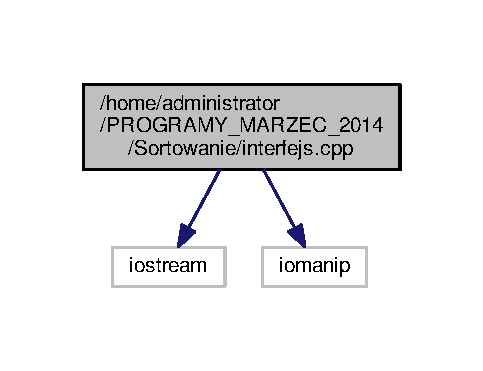
\includegraphics[width=232pt]{interfejs_8cpp__incl}
\end{center}
\end{figure}
\subsection*{Funkcje}
\begin{DoxyCompactItemize}
\item 
void \hyperlink{interfejs_8cpp_a11e0f29641d739b7317d5ac56347f7dd}{W\+Y\+P\+I\+S\+Z\+\_\+\+O\+P\+C\+J\+A} ()
\begin{DoxyCompactList}\small\item\em Wypisuje tekst wyswietlany podczas wyboru opcji programu. \end{DoxyCompactList}\item 
void \hyperlink{interfejs_8cpp_af3c55047e56b3ffe909f0eab3f5f2a78}{W\+Y\+P\+I\+S\+Z\+\_\+\+W\+S\+T\+E\+P} ()
\begin{DoxyCompactList}\small\item\em Wypisuje tekst wyswietlany podczas startu programu. \end{DoxyCompactList}\item 
void \hyperlink{interfejs_8cpp_afe2e85b470420e3d401502187e92e527}{W\+Y\+P\+I\+S\+Z\+\_\+\+P\+A\+R\+A\+M\+E\+T\+R\+Y} (int ilosc\+\_\+elementow, double wstepnie\+\_\+posortowane, int Z\+A\+K\+R\+E\+S\+\_\+\+L\+O\+S\+O\+W\+A\+N\+I\+A)
\begin{DoxyCompactList}\small\item\em Wypisanie na ekranie aktualnie ustawionych parametrow programu. \end{DoxyCompactList}\item 
void \hyperlink{interfejs_8cpp_a1500e9c6dc085ca4f77a989603aa3035}{W\+Y\+P\+I\+S\+Z\+\_\+\+M\+E\+N\+U} ()
\begin{DoxyCompactList}\small\item\em Wypisanie menu dostepnego dla uzytkownika. \end{DoxyCompactList}\item 
void \hyperlink{interfejs_8cpp_a7de2662a16e6ea5d4d207fddd44b3e56}{W\+Y\+P\+I\+S\+Z\+\_\+\+I\+L\+O\+S\+C\+\_\+\+E\+L\+E\+M\+E\+N\+T\+O\+W} ()
\begin{DoxyCompactList}\small\item\em Wypisanie \char`\"{}menu\char`\"{} wyboru ilosci elementow. \end{DoxyCompactList}\item 
void \hyperlink{interfejs_8cpp_ad25ada030bf26a8e1b25f9f8b2610fdf}{W\+Y\+P\+I\+S\+Z\+\_\+\+W\+S\+T\+E\+P\+N\+I\+E\+\_\+\+P\+O\+S\+O\+R\+T\+O\+W\+A\+N\+E} ()
\begin{DoxyCompactList}\small\item\em Wypisanie \char`\"{}menu\char`\"{} wyboru opcji wstepnie posortowanych elementow. \end{DoxyCompactList}\end{DoxyCompactItemize}


\subsection{Dokumentacja funkcji}
\hypertarget{interfejs_8cpp_a7de2662a16e6ea5d4d207fddd44b3e56}{\index{interfejs.\+cpp@{interfejs.\+cpp}!W\+Y\+P\+I\+S\+Z\+\_\+\+I\+L\+O\+S\+C\+\_\+\+E\+L\+E\+M\+E\+N\+T\+O\+W@{W\+Y\+P\+I\+S\+Z\+\_\+\+I\+L\+O\+S\+C\+\_\+\+E\+L\+E\+M\+E\+N\+T\+O\+W}}
\index{W\+Y\+P\+I\+S\+Z\+\_\+\+I\+L\+O\+S\+C\+\_\+\+E\+L\+E\+M\+E\+N\+T\+O\+W@{W\+Y\+P\+I\+S\+Z\+\_\+\+I\+L\+O\+S\+C\+\_\+\+E\+L\+E\+M\+E\+N\+T\+O\+W}!interfejs.\+cpp@{interfejs.\+cpp}}
\subsubsection[{W\+Y\+P\+I\+S\+Z\+\_\+\+I\+L\+O\+S\+C\+\_\+\+E\+L\+E\+M\+E\+N\+T\+O\+W}]{\setlength{\rightskip}{0pt plus 5cm}void W\+Y\+P\+I\+S\+Z\+\_\+\+I\+L\+O\+S\+C\+\_\+\+E\+L\+E\+M\+E\+N\+T\+O\+W (
\begin{DoxyParamCaption}
{}
\end{DoxyParamCaption}
)}}\label{interfejs_8cpp_a7de2662a16e6ea5d4d207fddd44b3e56}


Wypisanie \char`\"{}menu\char`\"{} wyboru ilosci elementow. 

\hypertarget{interfejs_8cpp_a1500e9c6dc085ca4f77a989603aa3035}{\index{interfejs.\+cpp@{interfejs.\+cpp}!W\+Y\+P\+I\+S\+Z\+\_\+\+M\+E\+N\+U@{W\+Y\+P\+I\+S\+Z\+\_\+\+M\+E\+N\+U}}
\index{W\+Y\+P\+I\+S\+Z\+\_\+\+M\+E\+N\+U@{W\+Y\+P\+I\+S\+Z\+\_\+\+M\+E\+N\+U}!interfejs.\+cpp@{interfejs.\+cpp}}
\subsubsection[{W\+Y\+P\+I\+S\+Z\+\_\+\+M\+E\+N\+U}]{\setlength{\rightskip}{0pt plus 5cm}void W\+Y\+P\+I\+S\+Z\+\_\+\+M\+E\+N\+U (
\begin{DoxyParamCaption}
{}
\end{DoxyParamCaption}
)}}\label{interfejs_8cpp_a1500e9c6dc085ca4f77a989603aa3035}


Wypisanie menu dostepnego dla uzytkownika. 

\hypertarget{interfejs_8cpp_a11e0f29641d739b7317d5ac56347f7dd}{\index{interfejs.\+cpp@{interfejs.\+cpp}!W\+Y\+P\+I\+S\+Z\+\_\+\+O\+P\+C\+J\+A@{W\+Y\+P\+I\+S\+Z\+\_\+\+O\+P\+C\+J\+A}}
\index{W\+Y\+P\+I\+S\+Z\+\_\+\+O\+P\+C\+J\+A@{W\+Y\+P\+I\+S\+Z\+\_\+\+O\+P\+C\+J\+A}!interfejs.\+cpp@{interfejs.\+cpp}}
\subsubsection[{W\+Y\+P\+I\+S\+Z\+\_\+\+O\+P\+C\+J\+A}]{\setlength{\rightskip}{0pt plus 5cm}void W\+Y\+P\+I\+S\+Z\+\_\+\+O\+P\+C\+J\+A (
\begin{DoxyParamCaption}
{}
\end{DoxyParamCaption}
)}}\label{interfejs_8cpp_a11e0f29641d739b7317d5ac56347f7dd}


Wypisuje tekst wyswietlany podczas wyboru opcji programu. 

\hypertarget{interfejs_8cpp_afe2e85b470420e3d401502187e92e527}{\index{interfejs.\+cpp@{interfejs.\+cpp}!W\+Y\+P\+I\+S\+Z\+\_\+\+P\+A\+R\+A\+M\+E\+T\+R\+Y@{W\+Y\+P\+I\+S\+Z\+\_\+\+P\+A\+R\+A\+M\+E\+T\+R\+Y}}
\index{W\+Y\+P\+I\+S\+Z\+\_\+\+P\+A\+R\+A\+M\+E\+T\+R\+Y@{W\+Y\+P\+I\+S\+Z\+\_\+\+P\+A\+R\+A\+M\+E\+T\+R\+Y}!interfejs.\+cpp@{interfejs.\+cpp}}
\subsubsection[{W\+Y\+P\+I\+S\+Z\+\_\+\+P\+A\+R\+A\+M\+E\+T\+R\+Y}]{\setlength{\rightskip}{0pt plus 5cm}void W\+Y\+P\+I\+S\+Z\+\_\+\+P\+A\+R\+A\+M\+E\+T\+R\+Y (
\begin{DoxyParamCaption}
\item[{int}]{ilosc\+\_\+elementow, }
\item[{double}]{wstepnie\+\_\+posortowane, }
\item[{int}]{Z\+A\+K\+R\+E\+S\+\_\+\+S\+O\+R\+T\+O\+W\+A\+N\+I\+A}
\end{DoxyParamCaption}
)}}\label{interfejs_8cpp_afe2e85b470420e3d401502187e92e527}


Wypisanie na ekranie aktualnie ustawionych parametrow programu. 


\begin{DoxyParams}{Parametry}
{\em ilosc\+\_\+elementow} & -\/ aktualnie ustawiona ilosc elementow \\
\hline
{\em wstepnie\+\_\+posortowane} & -\/ ilosc wstepnie posortowanych elementow \\
\hline
{\em Z\+A\+K\+R\+E\+S\+\_\+\+S\+O\+R\+T\+O\+W\+A\+N\+I\+A} & -\/ zakres, z ktorego losowane beda liczby \\
\hline
\end{DoxyParams}
\hypertarget{interfejs_8cpp_af3c55047e56b3ffe909f0eab3f5f2a78}{\index{interfejs.\+cpp@{interfejs.\+cpp}!W\+Y\+P\+I\+S\+Z\+\_\+\+W\+S\+T\+E\+P@{W\+Y\+P\+I\+S\+Z\+\_\+\+W\+S\+T\+E\+P}}
\index{W\+Y\+P\+I\+S\+Z\+\_\+\+W\+S\+T\+E\+P@{W\+Y\+P\+I\+S\+Z\+\_\+\+W\+S\+T\+E\+P}!interfejs.\+cpp@{interfejs.\+cpp}}
\subsubsection[{W\+Y\+P\+I\+S\+Z\+\_\+\+W\+S\+T\+E\+P}]{\setlength{\rightskip}{0pt plus 5cm}void W\+Y\+P\+I\+S\+Z\+\_\+\+W\+S\+T\+E\+P (
\begin{DoxyParamCaption}
{}
\end{DoxyParamCaption}
)}}\label{interfejs_8cpp_af3c55047e56b3ffe909f0eab3f5f2a78}


Wypisuje tekst wyswietlany podczas startu programu. 

\hypertarget{interfejs_8cpp_ad25ada030bf26a8e1b25f9f8b2610fdf}{\index{interfejs.\+cpp@{interfejs.\+cpp}!W\+Y\+P\+I\+S\+Z\+\_\+\+W\+S\+T\+E\+P\+N\+I\+E\+\_\+\+P\+O\+S\+O\+R\+T\+O\+W\+A\+N\+E@{W\+Y\+P\+I\+S\+Z\+\_\+\+W\+S\+T\+E\+P\+N\+I\+E\+\_\+\+P\+O\+S\+O\+R\+T\+O\+W\+A\+N\+E}}
\index{W\+Y\+P\+I\+S\+Z\+\_\+\+W\+S\+T\+E\+P\+N\+I\+E\+\_\+\+P\+O\+S\+O\+R\+T\+O\+W\+A\+N\+E@{W\+Y\+P\+I\+S\+Z\+\_\+\+W\+S\+T\+E\+P\+N\+I\+E\+\_\+\+P\+O\+S\+O\+R\+T\+O\+W\+A\+N\+E}!interfejs.\+cpp@{interfejs.\+cpp}}
\subsubsection[{W\+Y\+P\+I\+S\+Z\+\_\+\+W\+S\+T\+E\+P\+N\+I\+E\+\_\+\+P\+O\+S\+O\+R\+T\+O\+W\+A\+N\+E}]{\setlength{\rightskip}{0pt plus 5cm}void W\+Y\+P\+I\+S\+Z\+\_\+\+W\+S\+T\+E\+P\+N\+I\+E\+\_\+\+P\+O\+S\+O\+R\+T\+O\+W\+A\+N\+E (
\begin{DoxyParamCaption}
{}
\end{DoxyParamCaption}
)}}\label{interfejs_8cpp_ad25ada030bf26a8e1b25f9f8b2610fdf}


Wypisanie \char`\"{}menu\char`\"{} wyboru opcji wstepnie posortowanych elementow. 


\hypertarget{interfejs_8h}{\section{Dokumentacja pliku /home/administrator/\+P\+R\+O\+G\+R\+A\+M\+Y\+\_\+\+M\+A\+R\+Z\+E\+C\+\_\+2014/\+Sortowanie/interfejs.h}
\label{interfejs_8h}\index{/home/administrator/\+P\+R\+O\+G\+R\+A\+M\+Y\+\_\+\+M\+A\+R\+Z\+E\+C\+\_\+2014/\+Sortowanie/interfejs.\+h@{/home/administrator/\+P\+R\+O\+G\+R\+A\+M\+Y\+\_\+\+M\+A\+R\+Z\+E\+C\+\_\+2014/\+Sortowanie/interfejs.\+h}}
}
Ten wykres pokazuje, które pliki bezpośrednio lub pośrednio załączają ten plik\+:
\nopagebreak
\begin{figure}[H]
\begin{center}
\leavevmode
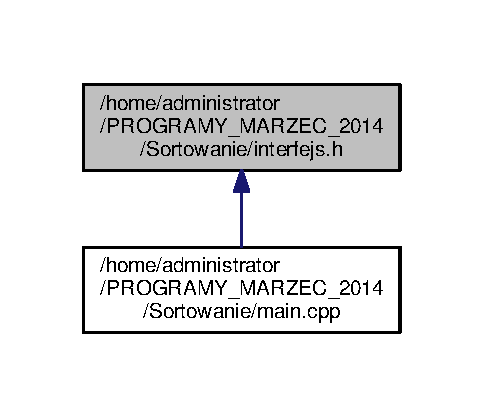
\includegraphics[width=232pt]{interfejs_8h__dep__incl}
\end{center}
\end{figure}
\subsection*{Funkcje}
\begin{DoxyCompactItemize}
\item 
void \hyperlink{interfejs_8h_a11e0f29641d739b7317d5ac56347f7dd}{W\+Y\+P\+I\+S\+Z\+\_\+\+O\+P\+C\+J\+A} ()
\begin{DoxyCompactList}\small\item\em Wypisuje tekst wyswietlany podczas wyboru opcji programu. \end{DoxyCompactList}\item 
void \hyperlink{interfejs_8h_af3c55047e56b3ffe909f0eab3f5f2a78}{W\+Y\+P\+I\+S\+Z\+\_\+\+W\+S\+T\+E\+P} ()
\begin{DoxyCompactList}\small\item\em Wypisuje tekst wyswietlany podczas startu programu. \end{DoxyCompactList}\item 
void \hyperlink{interfejs_8h_ae97ed87500f5be179d98f8686cecabc1}{W\+Y\+P\+I\+S\+Z\+\_\+\+P\+A\+R\+A\+M\+E\+T\+R\+Y} (int ilosc\+\_\+elementow, double wstepnie\+\_\+posortowane, int Z\+A\+K\+R\+E\+S\+\_\+\+S\+O\+R\+T\+O\+W\+A\+N\+I\+A)
\begin{DoxyCompactList}\small\item\em Wypisanie na ekranie aktualnie ustawionych parametrow programu. \end{DoxyCompactList}\item 
void \hyperlink{interfejs_8h_a1500e9c6dc085ca4f77a989603aa3035}{W\+Y\+P\+I\+S\+Z\+\_\+\+M\+E\+N\+U} ()
\begin{DoxyCompactList}\small\item\em Wypisanie menu dostepnego dla uzytkownika. \end{DoxyCompactList}\item 
void \hyperlink{interfejs_8h_a7de2662a16e6ea5d4d207fddd44b3e56}{W\+Y\+P\+I\+S\+Z\+\_\+\+I\+L\+O\+S\+C\+\_\+\+E\+L\+E\+M\+E\+N\+T\+O\+W} ()
\begin{DoxyCompactList}\small\item\em Wypisanie \char`\"{}menu\char`\"{} wyboru ilosci elementow. \end{DoxyCompactList}\item 
void \hyperlink{interfejs_8h_ad25ada030bf26a8e1b25f9f8b2610fdf}{W\+Y\+P\+I\+S\+Z\+\_\+\+W\+S\+T\+E\+P\+N\+I\+E\+\_\+\+P\+O\+S\+O\+R\+T\+O\+W\+A\+N\+E} ()
\begin{DoxyCompactList}\small\item\em Wypisanie \char`\"{}menu\char`\"{} wyboru opcji wstepnie posortowanych elementow. \end{DoxyCompactList}\end{DoxyCompactItemize}


\subsection{Dokumentacja funkcji}
\hypertarget{interfejs_8h_a7de2662a16e6ea5d4d207fddd44b3e56}{\index{interfejs.\+h@{interfejs.\+h}!W\+Y\+P\+I\+S\+Z\+\_\+\+I\+L\+O\+S\+C\+\_\+\+E\+L\+E\+M\+E\+N\+T\+O\+W@{W\+Y\+P\+I\+S\+Z\+\_\+\+I\+L\+O\+S\+C\+\_\+\+E\+L\+E\+M\+E\+N\+T\+O\+W}}
\index{W\+Y\+P\+I\+S\+Z\+\_\+\+I\+L\+O\+S\+C\+\_\+\+E\+L\+E\+M\+E\+N\+T\+O\+W@{W\+Y\+P\+I\+S\+Z\+\_\+\+I\+L\+O\+S\+C\+\_\+\+E\+L\+E\+M\+E\+N\+T\+O\+W}!interfejs.\+h@{interfejs.\+h}}
\subsubsection[{W\+Y\+P\+I\+S\+Z\+\_\+\+I\+L\+O\+S\+C\+\_\+\+E\+L\+E\+M\+E\+N\+T\+O\+W}]{\setlength{\rightskip}{0pt plus 5cm}void W\+Y\+P\+I\+S\+Z\+\_\+\+I\+L\+O\+S\+C\+\_\+\+E\+L\+E\+M\+E\+N\+T\+O\+W (
\begin{DoxyParamCaption}
{}
\end{DoxyParamCaption}
)}}\label{interfejs_8h_a7de2662a16e6ea5d4d207fddd44b3e56}


Wypisanie \char`\"{}menu\char`\"{} wyboru ilosci elementow. 

\hypertarget{interfejs_8h_a1500e9c6dc085ca4f77a989603aa3035}{\index{interfejs.\+h@{interfejs.\+h}!W\+Y\+P\+I\+S\+Z\+\_\+\+M\+E\+N\+U@{W\+Y\+P\+I\+S\+Z\+\_\+\+M\+E\+N\+U}}
\index{W\+Y\+P\+I\+S\+Z\+\_\+\+M\+E\+N\+U@{W\+Y\+P\+I\+S\+Z\+\_\+\+M\+E\+N\+U}!interfejs.\+h@{interfejs.\+h}}
\subsubsection[{W\+Y\+P\+I\+S\+Z\+\_\+\+M\+E\+N\+U}]{\setlength{\rightskip}{0pt plus 5cm}void W\+Y\+P\+I\+S\+Z\+\_\+\+M\+E\+N\+U (
\begin{DoxyParamCaption}
{}
\end{DoxyParamCaption}
)}}\label{interfejs_8h_a1500e9c6dc085ca4f77a989603aa3035}


Wypisanie menu dostepnego dla uzytkownika. 

\hypertarget{interfejs_8h_a11e0f29641d739b7317d5ac56347f7dd}{\index{interfejs.\+h@{interfejs.\+h}!W\+Y\+P\+I\+S\+Z\+\_\+\+O\+P\+C\+J\+A@{W\+Y\+P\+I\+S\+Z\+\_\+\+O\+P\+C\+J\+A}}
\index{W\+Y\+P\+I\+S\+Z\+\_\+\+O\+P\+C\+J\+A@{W\+Y\+P\+I\+S\+Z\+\_\+\+O\+P\+C\+J\+A}!interfejs.\+h@{interfejs.\+h}}
\subsubsection[{W\+Y\+P\+I\+S\+Z\+\_\+\+O\+P\+C\+J\+A}]{\setlength{\rightskip}{0pt plus 5cm}void W\+Y\+P\+I\+S\+Z\+\_\+\+O\+P\+C\+J\+A (
\begin{DoxyParamCaption}
{}
\end{DoxyParamCaption}
)}}\label{interfejs_8h_a11e0f29641d739b7317d5ac56347f7dd}


Wypisuje tekst wyswietlany podczas wyboru opcji programu. 

\hypertarget{interfejs_8h_ae97ed87500f5be179d98f8686cecabc1}{\index{interfejs.\+h@{interfejs.\+h}!W\+Y\+P\+I\+S\+Z\+\_\+\+P\+A\+R\+A\+M\+E\+T\+R\+Y@{W\+Y\+P\+I\+S\+Z\+\_\+\+P\+A\+R\+A\+M\+E\+T\+R\+Y}}
\index{W\+Y\+P\+I\+S\+Z\+\_\+\+P\+A\+R\+A\+M\+E\+T\+R\+Y@{W\+Y\+P\+I\+S\+Z\+\_\+\+P\+A\+R\+A\+M\+E\+T\+R\+Y}!interfejs.\+h@{interfejs.\+h}}
\subsubsection[{W\+Y\+P\+I\+S\+Z\+\_\+\+P\+A\+R\+A\+M\+E\+T\+R\+Y}]{\setlength{\rightskip}{0pt plus 5cm}void W\+Y\+P\+I\+S\+Z\+\_\+\+P\+A\+R\+A\+M\+E\+T\+R\+Y (
\begin{DoxyParamCaption}
\item[{int}]{ilosc\+\_\+elementow, }
\item[{double}]{wstepnie\+\_\+posortowane, }
\item[{int}]{Z\+A\+K\+R\+E\+S\+\_\+\+S\+O\+R\+T\+O\+W\+A\+N\+I\+A}
\end{DoxyParamCaption}
)}}\label{interfejs_8h_ae97ed87500f5be179d98f8686cecabc1}


Wypisanie na ekranie aktualnie ustawionych parametrow programu. 


\begin{DoxyParams}{Parametry}
{\em ilosc\+\_\+elementow} & -\/ aktualnie ustawiona ilosc elementow \\
\hline
{\em wstepnie\+\_\+posortowane} & -\/ ilosc wstepnie posortowanych elementow \\
\hline
{\em Z\+A\+K\+R\+E\+S\+\_\+\+S\+O\+R\+T\+O\+W\+A\+N\+I\+A} & -\/ zakres, z ktorego losowane beda liczby \\
\hline
\end{DoxyParams}
\hypertarget{interfejs_8h_af3c55047e56b3ffe909f0eab3f5f2a78}{\index{interfejs.\+h@{interfejs.\+h}!W\+Y\+P\+I\+S\+Z\+\_\+\+W\+S\+T\+E\+P@{W\+Y\+P\+I\+S\+Z\+\_\+\+W\+S\+T\+E\+P}}
\index{W\+Y\+P\+I\+S\+Z\+\_\+\+W\+S\+T\+E\+P@{W\+Y\+P\+I\+S\+Z\+\_\+\+W\+S\+T\+E\+P}!interfejs.\+h@{interfejs.\+h}}
\subsubsection[{W\+Y\+P\+I\+S\+Z\+\_\+\+W\+S\+T\+E\+P}]{\setlength{\rightskip}{0pt plus 5cm}void W\+Y\+P\+I\+S\+Z\+\_\+\+W\+S\+T\+E\+P (
\begin{DoxyParamCaption}
{}
\end{DoxyParamCaption}
)}}\label{interfejs_8h_af3c55047e56b3ffe909f0eab3f5f2a78}


Wypisuje tekst wyswietlany podczas startu programu. 

\hypertarget{interfejs_8h_ad25ada030bf26a8e1b25f9f8b2610fdf}{\index{interfejs.\+h@{interfejs.\+h}!W\+Y\+P\+I\+S\+Z\+\_\+\+W\+S\+T\+E\+P\+N\+I\+E\+\_\+\+P\+O\+S\+O\+R\+T\+O\+W\+A\+N\+E@{W\+Y\+P\+I\+S\+Z\+\_\+\+W\+S\+T\+E\+P\+N\+I\+E\+\_\+\+P\+O\+S\+O\+R\+T\+O\+W\+A\+N\+E}}
\index{W\+Y\+P\+I\+S\+Z\+\_\+\+W\+S\+T\+E\+P\+N\+I\+E\+\_\+\+P\+O\+S\+O\+R\+T\+O\+W\+A\+N\+E@{W\+Y\+P\+I\+S\+Z\+\_\+\+W\+S\+T\+E\+P\+N\+I\+E\+\_\+\+P\+O\+S\+O\+R\+T\+O\+W\+A\+N\+E}!interfejs.\+h@{interfejs.\+h}}
\subsubsection[{W\+Y\+P\+I\+S\+Z\+\_\+\+W\+S\+T\+E\+P\+N\+I\+E\+\_\+\+P\+O\+S\+O\+R\+T\+O\+W\+A\+N\+E}]{\setlength{\rightskip}{0pt plus 5cm}void W\+Y\+P\+I\+S\+Z\+\_\+\+W\+S\+T\+E\+P\+N\+I\+E\+\_\+\+P\+O\+S\+O\+R\+T\+O\+W\+A\+N\+E (
\begin{DoxyParamCaption}
{}
\end{DoxyParamCaption}
)}}\label{interfejs_8h_ad25ada030bf26a8e1b25f9f8b2610fdf}


Wypisanie \char`\"{}menu\char`\"{} wyboru opcji wstepnie posortowanych elementow. 


\hypertarget{main_8cpp}{\section{Dokumentacja pliku /home/administrator/\+P\+R\+O\+G\+R\+A\+M\+Y\+\_\+\+M\+A\+R\+Z\+E\+C\+\_\+2014/\+Sortowanie/main.cpp}
\label{main_8cpp}\index{/home/administrator/\+P\+R\+O\+G\+R\+A\+M\+Y\+\_\+\+M\+A\+R\+Z\+E\+C\+\_\+2014/\+Sortowanie/main.\+cpp@{/home/administrator/\+P\+R\+O\+G\+R\+A\+M\+Y\+\_\+\+M\+A\+R\+Z\+E\+C\+\_\+2014/\+Sortowanie/main.\+cpp}}
}
{\ttfamily \#include $<$iostream$>$}\\*
{\ttfamily \#include $<$cstdlib$>$}\\*
{\ttfamily \#include $<$ctime$>$}\\*
{\ttfamily \#include $<$iomanip$>$}\\*
{\ttfamily \#include $<$cmath$>$}\\*
{\ttfamily \#include \char`\"{}interfejs.\+h\char`\"{}}\\*
{\ttfamily \#include \char`\"{}funkcje.\+h\char`\"{}}\\*
Wykres zależności załączania dla main.\+cpp\+:
\nopagebreak
\begin{figure}[H]
\begin{center}
\leavevmode
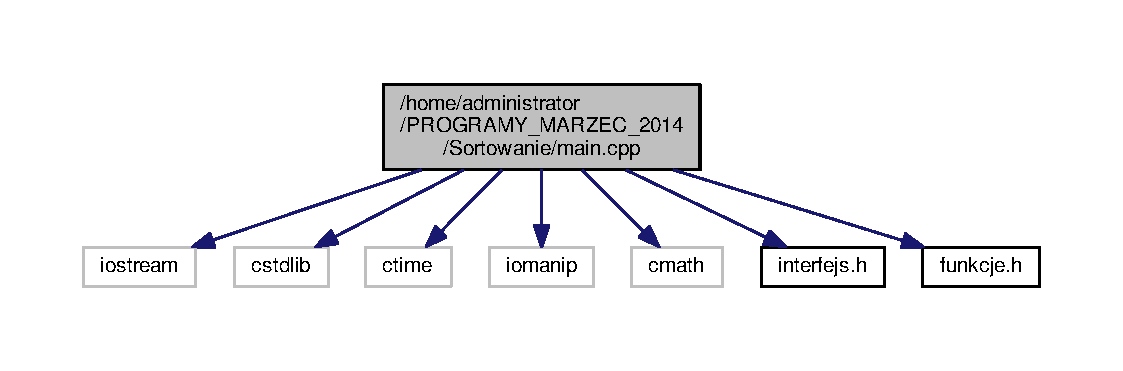
\includegraphics[width=350pt]{main_8cpp__incl}
\end{center}
\end{figure}
\subsection*{Definicje}
\begin{DoxyCompactItemize}
\item 
\#define \hyperlink{main_8cpp_aa50aa866c5823769bb02e986d29a0589}{R\+O\+Z\+M\+I\+A\+R}~100
\end{DoxyCompactItemize}
\subsection*{Funkcje}
\begin{DoxyCompactItemize}
\item 
int \hyperlink{main_8cpp_ae66f6b31b5ad750f1fe042a706a4e3d4}{main} ()
\end{DoxyCompactItemize}


\subsection{Dokumentacja definicji}
\hypertarget{main_8cpp_aa50aa866c5823769bb02e986d29a0589}{\index{main.\+cpp@{main.\+cpp}!R\+O\+Z\+M\+I\+A\+R@{R\+O\+Z\+M\+I\+A\+R}}
\index{R\+O\+Z\+M\+I\+A\+R@{R\+O\+Z\+M\+I\+A\+R}!main.\+cpp@{main.\+cpp}}
\subsubsection[{R\+O\+Z\+M\+I\+A\+R}]{\setlength{\rightskip}{0pt plus 5cm}\#define R\+O\+Z\+M\+I\+A\+R~100}}\label{main_8cpp_aa50aa866c5823769bb02e986d29a0589}
$^\wedge$$^\wedge$$^\wedge$$^\wedge$$^\wedge$$^\wedge$$^\wedge$$^\wedge$$^\wedge$$^\wedge$$^\wedge$$^\wedge$$^\wedge$$^\wedge$$^\wedge$$^\wedge$$^\wedge$$^\wedge$$^\wedge$$^\wedge$$^\wedge$$^\wedge$$^\wedge$$^\wedge$$^\wedge$$^\wedge$$^\wedge$$^\wedge$$^\wedge$$^\wedge$$^\wedge$$^\wedge$$^\wedge$$^\wedge$$^\wedge$$^\wedge$$^\wedge$$^\wedge$$^\wedge$ Testy algorytmow sortowania Autor\+: Bizon Michal \subsubsection*{Indeks\+: 195251 }

Aby przetestowac dzialanie algorytmow (D\+E\+B\+U\+G), nalezy zmienic wartosc nr 1 tabeli \char`\"{}const int ilosc\+\_\+elementow\char`\"{} na 100 i odkomentowac petle for po kazdym sortowaniu, tudziez po stworzeniu tablicy. Dla wygody uzytkownika wyswietlany jest tylko pierwszy wiersz calej tablicy (wyswietlanie 100 wierszy po 100 elementow czterokrotnie (po kazdym sortowaniu) byloby uciazliwe).

Program dla kazdej partii sortowan (tj wszystkich 4) uzywa tablicy z tymi samymi wartosciami, aby testy byly wiarygodne. Dlatego zostaly stworzone dwie tablice -\/ jedna bazowa -\/ T\+A\+B\+L\+I\+C\+A, przechowuje pierwotna tablice, druga pomocnicza -\/ do ktorej przypisywane sa pierwotne wartosci po kazdym sortowaniu, a dopiero pozniej sa sortowane.

Pomiar czasu jest dokonywany z dokladnoscia do 0.\+001 \mbox{[}s\mbox{]}, co w przypadku malych tablic jest niezbyt dokladne, jednak przy wiekszych spelnia swoje zadanie.

Dla wygody przeprowadzenia analiz dane dotyczace czasow sortowan sa zapisywane do pliku tekstowego z pseudo-\/formatowaniem

Mimo iz rozwiazanie jakie zastosowalem (odnosnie przesylania i sortowania jednego wiersza funkcji) nie jest idealne, ale pozwala na dokladny pomiar czasu oraz wygodne zarzadzanie pamiecia. 

\subsection{Dokumentacja funkcji}
\hypertarget{main_8cpp_ae66f6b31b5ad750f1fe042a706a4e3d4}{\index{main.\+cpp@{main.\+cpp}!main@{main}}
\index{main@{main}!main.\+cpp@{main.\+cpp}}
\subsubsection[{main}]{\setlength{\rightskip}{0pt plus 5cm}int main (
\begin{DoxyParamCaption}
{}
\end{DoxyParamCaption}
)}}\label{main_8cpp_ae66f6b31b5ad750f1fe042a706a4e3d4}
Glowna tablica -\/ \mbox{[}\char`\"{}\+R\+O\+Z\+M\+I\+A\+R\char`\"{} wierszy\mbox{]} X \mbox{[}\char`\"{}ilosc\+\_\+elementow\char`\"{} kolumn\mbox{]}

Wykozystanie tej samej tablicy dla kazdego sortowania

Tablica pomocnicza wysylana do funkcji sortowania przez scalanie

Aby bez problemow zapisac dane do pliku umiescilem je w tabeli

Sumy takze

sterowanie opcjami programu

rozmiar kazdego wiersza w tablicy

ilosc wstepnie posortowanych elementow

Zakres (0-\/x), z ktorego uzytkownik losuje liczby

Sterowanie glownym menu -\/ do petli switch

Zliczanie czasu pomiedzy wykonaniem sie operacji

oraz roznica miedzy nimi

Introspektywne -\/ aby odroznic kiedy qiucksort ma dzialac samodzielnie a kiedy jedynie partycjonowac tablice dla introsorta

Wypisanie interfejsu graficznego programu oraz

parametrow symulacji

Wypisanie dostepnych opcji wyboru

Maksymalna wartoscia jest 4

Zadeklarowanie wielkosci tablic T\+A\+B\+\_\+\+P\+O\+M i T\+A\+B\+E\+L\+A\+\_\+\+S\+O\+R\+T\+O\+W\+A\+N dla danego \char`\"{}przebiegu\char`\"{} funkcji -\/ wypelniane N\+U\+L\+L'ami

Budowanie T\+A\+B\+L\+I\+C\+Y Na podstawie parametrow wylicza ile elementow ma byc posortowane poczatkowo, jezeli wartosc \char`\"{}ile\+\_\+posortowac\char`\"{} wynosi 0, to program najpierw sortuje tablice za pomoca Sortowania przez Scalanie, a nastepnie odwraca tabele (pierwszy z ostatnim itd) funkcja swap(\+A\mbox{[}n\mbox{]},\+A\mbox{[}m\mbox{]}).

W innym wypadku funkcja wylicza, jakie wartosci powinny byc z danego zakresu (np 25\% z 1000 to 250), losuje liczby z tego przedzia�u, sortuje je, a nastepnie losuje liczby z zakresu 250-\/1000.

Zmienna i jest przekazana aby rand by� lepszy, tj aby nie bylo obok siebie (np T\+A\+B\+L\+I\+C\+A\mbox{[}0\mbox{]} i T\+A\+B\+L\+I\+C\+A\mbox{[}1\mbox{]}) takich samych wartosci randa generowanego na podstawie aktualnego czasu



 Algorytmy S\+O\+R\+T\+O\+W\+A\+N\+I\+A 

 Sortowanie przez S\+C\+A\+L\+A\+N\+I\+E

Sortowanie S\+Z\+Y\+B\+K\+I\+E

Sortowanie I\+N\+T\+R\+O\+S\+P\+E\+K\+T\+Y\+W\+N\+E

Sortowanie przez Kopcowanie 
%--- End generated contents ---

% Index
\newpage
\phantomsection
\addcontentsline{toc}{chapter}{Indeks}
\printindex

\end{document}
